\documentclass[11pt,a4paper]{article}
\usepackage[utf8]{inputenc}
\usepackage[T1]{fontenc}
\usepackage{geometry}
\usepackage{setspace}
\usepackage{parskip}
\usepackage{amsmath,amssymb}
\usepackage{graphicx}
\usepackage{booktabs}
\usepackage{array}
\usepackage{longtable}
\usepackage{enumitem}
\usepackage{xcolor}
\usepackage{hyperref}
\usepackage{float}
\usepackage{fancyhdr}
\usepackage{titlesec}
\usepackage{pdflscape}
\usepackage{tikz}
\usetikzlibrary{positioning,arrows.meta}

\geometry{left=2.5cm,right=2.5cm,top=2.5cm,bottom=2.5cm,headheight=14.5pt}
\onehalfspacing
\hypersetup{
    colorlinks=true, linkcolor=black, urlcolor=blue, citecolor=black,
    pdftitle={Descripción de la Arquitectura del Software (SAD) - Sistema Integral de Gestión de Eventos},
    pdfauthor={Hexacore}, hidelinks=false
}

\definecolor{azul}{RGB}{31,78,121}
\definecolor{gris}{RGB}{242,242,242}
\definecolor{grisoscuro}{RGB}{80,80,80}

\renewcommand{\figurename}{Figura}
\renewcommand{\tablename}{Tabla}

\newcommand{\pendiente}[1]{\textit{\textcolor{grisoscuro}{[Pendiente: #1]}}}
\setlist[itemize]{topsep=2pt, itemsep=2pt}

\titleformat{\section}{\Large\bfseries\color{azul}}{\thesection.}{0.5em}{}
\titleformat{\subsection}{\large\bfseries}{\thesubsection.}{0.5em}{}

\pagestyle{fancy}
\fancyhf{}
\fancyhead[L]{Sistema Integral de Gestión de Eventos}
\fancyhead[R]{\small Descripción de la Arquitectura del Software (SAD)}
\fancyfoot[C]{\thepage}
\renewcommand{\headrulewidth}{0.4pt}

\newcolumntype{P}[1]{>{\raggedright\arraybackslash}p{#1}}

\title{\textbf{Descripción de la Arquitectura del Software (SAD)}}
\author{}
\date{}

\begin{document}

% ==================== Portada ====================
\begin{titlepage}
\centering
\vspace*{2cm}
{\LARGE \textbf{Descripción de la Arquitectura del Software (SAD)}}\\[0.4cm]
{\Large Sistema Integral de Gestión de Eventos}\\[1.5cm]
{\Large Equipo Hexacore}\\[2cm]
{\large Versión: 1.1}\\[0.5cm]
{\large Fecha de entrega: 27/08/2026}\\[2cm]
{\large Autores:}\\
{\large Daniel Cristancho}\\
{\large Samuel Emperador}\\
{\large Sebastián Sánchez}\\
{\large Diego Coronado}\\
\vfill
{\small Materia: Arquitectura de Software}
\end{titlepage}

% ==================== Historial de cambios ====================
\section*{Historial de Cambios}
\addcontentsline{toc}{section}{Historial de Cambios}

\begin{center}
\begin{longtable}{|p{2.5cm}|p{7cm}|p{4cm}|}
\hline
\textbf{Fecha} & \textbf{Descripción del cambio} & \textbf{Persona(s)} \\
\hline
\endhead
25/08/2026 & Creación de la versión 1.0 del documento, consolidando el trabajo ya elaborado en
\textit{ArchitecturalProposal.tex} (atributos de calidad y propuesta arquitectónica),
\textit{C4Diagrams.tex} (los seis diagramas C4), \textit{Submission/DistribucionCasosUso.pdf} (los
32 casos de uso) y \textit{BitacoraArquitectonica.md} (decisiones, alternativas y riesgos). Se añade
además un primer Árbol de Utilidad (ASR) y los ADR de las decisiones fundacionales, que hasta
ahora solo existían en la bitácora. & Equipo Hexacore (vía asistente) \\
\hline
27/08/2026 & Versión 1.1: se cierran los puntos pendientes de la v1.0 — diagrama de clases UML
del modelo de dominio, vista de componentes de los contenedores Personal, Eventos/Emergencias y
Parqueaderos, ambientes de desarrollo y pruebas en la vista física, y modelo de datos detallado
por microservicio. & Equipo Hexacore (vía asistente) \\
\hline
28/08/2026 & Versión 1.2: durante la construcción del prototipo de la app móvil (Entrega 2) se
decide unificar \textbf{App Móvil del Cliente} y \textbf{App Móvil del Personal} en un único
contenedor \textbf{App Móvil}, que identifica el rol del usuario en el login y navega al conjunto
de pantallas correspondiente (ver ADR-07). Se actualiza la vista de contenedores (de cuatro a tres
interfaces desplegables) y ADR-02/ADR-05 en consecuencia. & Equipo Hexacore (vía asistente) \\
\hline
22/09/2026 & Versión 1.3: se añade la sección \textbf{Tácticas arquitectónicas por atributo de
calidad} (§\ref{sec:tacticas}), que dice cómo se realiza en el código cada atributo priorizado y
con qué medición se respalda. Cubre los cinco que la entrega exige demostrar en vivo: desempeño,
disponibilidad, \textbf{seguridad}, \textbf{consistencia} y desplegabilidad. Las cifras de la
columna «Evidencia medida» provienen de ejecutar los guiones de \texttt{pruebas/} contra el
sistema desplegado, no de estimaciones de diseño. & Equipo Hexacore (vía asistente) \\
\hline
\end{longtable}
\end{center}

% ==================== Tabla de contenidos ====================
\newpage
\renewcommand{\contentsname}{Tabla de Contenidos}
\tableofcontents
\thispagestyle{empty}
\newpage

% ==================== Introducción ====================
\section{Introducción}

El \textbf{Sistema Integral de Gestión de Eventos} centraliza en una sola plataforma los procesos
que hoy suelen estar dispersos en la organización de un evento masivo (conciertos, festivales,
partidos deportivos): venta de entradas y su mercado secundario, gestión de personal y turnos,
parqueaderos, pedidos y establecimientos de alimentos, logística y operación del evento, y la
administración general (usuarios, roles, recintos, proveedores, pagos y reportes). El problema
central que resuelve es la \textbf{ausencia de un sistema unificado} que coordine estos procesos
de forma consistente, segura y escalable, evitando información duplicada, errores humanos y falta
de trazabilidad, especialmente crítico cuando hay miles de asistentes concurrentes durante la
apertura de venta o el ingreso al recinto.

Los principales objetivos de negocio del sistema son: (1) permitir la venta y reventa segura de
entradas sin duplicar propietarios ni sobrevender localidades; (2) mantener la disponibilidad del
servicio durante los picos de tráfico propios de la apertura de venta, el ingreso masivo y las
emergencias; (3) dar trazabilidad y auditoría a las operaciones financieras y administrativas; y
(4) ofrecer una experiencia adecuada a cada tipo de usuario (cliente, personal operativo,
administración) sin que ninguna interfaz duplique lógica de negocio.

Los atributos de calidad de mayor prioridad para la arquitectura son \textbf{consistencia},
\textbf{disponibilidad}, \textbf{seguridad} y \textbf{rendimiento}, seguidos de \textbf{tiempo
real}, \textbf{escalabilidad} y \textbf{trazabilidad}; con prioridad baja-media se consideran
\textbf{usabilidad}, \textbf{mantenibilidad} y \textbf{portabilidad}. La sección
\ref{sec:asr} detalla estos atributos en formato de Árbol de Utilidad.

Este documento sigue la estructura estándar \textit{arc42} y se organiza así: primero se describen
los requisitos funcionales y el modelo de dominio (secciones \ref{sec:reqs}-\ref{sec:dominio}),
luego los interesados y los requisitos arquitectónicamente significativos (secciones
\ref{sec:stakeholders}-\ref{sec:asr}), después las restricciones del proyecto (sección
\ref{sec:restricciones}) y las vistas arquitectónicas C4 (contexto, contenedores, componentes,
procesos y física; secciones \ref{sec:contexto}-\ref{sec:fisica}), y finalmente el modelo de
datos, los registros de decisión (ADR), los riesgos técnicos, el glosario y las referencias.

% ==================== Requisitos funcionales ====================
\section{Visión general de los requisitos funcionales}
\label{sec:reqs}

El sistema define \textbf{32 casos de uso} (CU-001 a CU-032), cada uno con un identificador único
usado a lo largo de todo el documento. La especificación detallada de cada uno (actores, flujo
principal, flujos alternativos y excepciones) está en la hoja de cálculo
\textit{Submission/CU\_eventos\_completo.xlsx}; la Tabla \ref{tab:cu-bloques} resume los bloques
temáticos en los que se agrupan.

\begin{center}
\begin{longtable}{p{3.4cm}p{2.6cm}p{8.5cm}}
\toprule
\textbf{Bloque temático} & \textbf{Casos de uso} & \textbf{Alcance funcional}\\
\midrule
\endhead
Boletería / Compra de entradas & CU-001 -- CU-005 & Consulta de eventos, compra, validación de QR
en el ingreso, cancelaciones/devoluciones y promociones.\\[0.3em]
Mercado secundario y personal para eventos & CU-006 -- CU-010 & Reventa segura de entradas
(caso complejo), administración y asignación de personal, cambios de turno, registro de
asistencia y gestión de evacuación ante emergencias (caso complejo).\\[0.3em]
Pedidos y establecimientos de alimentos & CU-011 -- CU-015 & Pedido de alimentos durante el
evento, administración de menú/inventario, preparación y entrega validada por QR, y gestión de
los establecimientos.\\[0.3em]
Logística y operación del evento & CU-016 -- CU-020 & Planificación logística, asignación de
personal operativo, gestión de turno/asistencia en campo, monitoreo del evento y gestión de
incidentes.\\[0.3em]
Parqueaderos & CU-021 -- CU-025 & Reserva, ingreso/salida de vehículos, asignación de espacios,
cobro y control de ocupación.\\[0.3em]
Administración general (CRUD) & CU-026 -- CU-032 & Gestión de eventos, cuentas de usuario, roles
y permisos, recintos y zonas, proveedores, pagos/conciliación financiera, y reportes y
analítica.\\
\bottomrule
\caption{Bloques temáticos de los 32 casos de uso del sistema.}
\label{tab:cu-bloques}
\end{longtable}
\end{center}

Los casos de uso están repartidos entre los cuatro integrantes del equipo (8 por persona); esa
distribución, con nombre y descripción completa de cada CU, está documentada en
\textit{Submission/DistribucionCasosUso.pdf}. Dos casos de uso se destacan como los de mayor
complejidad arquitectónica y sirven de hilo conductor en las vistas de este documento:
\textbf{CU-006 (Gestión del Mercado Secundario de Entradas)} y \textbf{CU-010 (Gestionar
Evacuación ante Emergencias)}.

% ==================== Requisitos no funcionales ====================
\section{Requisitos No Funcionales (RNF)}
\label{sec:rnf}

Mientras los casos de uso de la sección anterior describen \textit{qué} hace el sistema, los
requisitos no funcionales describen \textit{con qué calidad} debe hacerlo. Cada RNF de la Tabla
\ref{tab:rnf} se deriva de uno de los atributos de calidad priorizados en
\textit{ArchitecturalProposal.tex} y se expresa con una \textbf{métrica y un umbral verificable},
de modo que pueda comprobarse objetivamente si se cumple o no --- un requisito redactado como
``el sistema debe ser rápido'' no es verificable y por lo tanto no se admite en esta tabla.

Los RNF son la entrada directa de las dos secciones siguientes: los
\textbf{ASR} (sección \ref{sec:asr}) seleccionan cuáles de estos requisitos tienen impacto
arquitectónico real, y el análisis de tácticas de \textit{ArchitecturalProposal.tex} justifica
con qué mecanismo se satisface cada uno.

\textbf{Nota sobre los umbrales.} Los valores numéricos son estimaciones razonadas del equipo a
partir de los escenarios del proyecto, no mediciones sobre un sistema en producción (que aún no
existe). Los umbrales de RNF-01 y RNF-02 se respaldan con las pruebas de concepto del proyecto
(véase \textit{App/PoCs/}); el resto se validará conforme se implemente cada dominio.

% La tabla vive en RequisitosNoFuncionales.tex, compartida con el SRS.
% ARCHIVO COMPARTIDO: la tabla de RNF vive aquí y la incluyen con \input tanto el SAD
% (DescripcionArquitecturaSoftware.tex) como el SRS (EspecificacionRequisitos.tex).
% Antes estaba copiada dentro del SAD; separarla evita que las dos versiones se
% separen a la primera corrección. Al editarla se actualizan los dos documentos.

\begin{center}
\begin{longtable}{p{1.3cm}p{5.2cm}p{2.4cm}p{5.4cm}}
\toprule
\textbf{ID} & \textbf{Requisito} & \textbf{Atributo} & \textbf{Métrica y umbral verificable}\\
\midrule
\endhead
RNF-01 & Ninguna entrada publicada en el mercado secundario puede venderse a dos compradores
(CU-006). & Consistencia & Ventas duplicadas bajo concurrencia: \textbf{0\%} con 50 intentos de
compra simultáneos sobre la misma publicación.\\[0.3em]
RNF-02 & Al transferirse una entrada, el QR anterior queda invalidado antes de emitir el nuevo
(CU-006). & Consistencia & Códigos QR antiguos aceptados en validación tras una transferencia:
\textbf{0}.\\[0.3em]
RNF-03 & El sistema sigue atendiendo solicitudes ante la caída de una instancia de cualquier
microservicio (CU-001--005, CU-002). & Disponibilidad & Disponibilidad mensual del API Gateway
\textbf{$\geq$ 99,9\%} (máx. 43 min de indisponibilidad al mes).\\[0.3em]
RNF-04 & Ante la caída de una instancia, el sistema se recupera sin intervención manual.
& Disponibilidad & Tiempo hasta volver a responder el 100\% de las solicitudes:
\textbf{$\leq$ 30 s}.\\[0.3em]
RNF-05 & El sistema nunca almacena datos completos de tarjetas de pago (CU-001, CU-011, CU-024).
& Seguridad & Campos de tarjeta persistidos en cualquier base de datos propia: \textbf{0}; el
cobro se delega íntegramente a la pasarela.\\[0.3em]
RNF-06 & Toda petición a un microservicio pasa autenticada y autorizada por rol desde el API
Gateway. & Seguridad & Endpoints de negocio alcanzables sin token válido: \textbf{0\%} sobre el
total de rutas expuestas.\\[0.3em]
RNF-07 & La consulta de disponibilidad de entradas responde con baja latencia durante la apertura
de venta (CU-001). & Rendimiento & Latencia \textbf{p95 $\leq$ 500 ms} con 2.000 usuarios
concurrentes.\\[0.3em]
RNF-08 & La validación del QR en el ingreso no genera filas perceptibles (CU-002, CU-005).
& Rendimiento & Latencia \textbf{p95 $\leq$ 300 ms} por validación.\\[0.3em]
RNF-09 & El aforo y la ocupación se reflejan casi de inmediato tras un ingreso o salida (CU-019,
CU-025). & Tiempo real & Retardo entre el evento y su reflejo en el tablero de monitoreo:
\textbf{$\leq$ 2 s}.\\[0.3em]
RNF-10 & El servicio de Entradas escala horizontalmente sin degradar los demás dominios (CU-001,
CU-006). & Escalabilidad & Al duplicar sus instancias, el throughput crece
\textbf{$\geq$ 1,7$\times$} (eficiencia $\geq$ 85\%) sin afectar la latencia de otros
servicios.\\[0.3em]
RNF-11 & Toda operación financiera queda auditada (CU-006, CU-031). & Trazabilidad & Operaciones
con registro completo (actor, marca de tiempo, id. de transacción, resultado): \textbf{100\%};
retención \textbf{$\geq$ 1 año}.\\[0.3em]
RNF-12 & Un cliente sin capacitación previa completa la compra de una entrada (CU-001).
& Usabilidad & \textbf{$\geq$ 80\%} de éxito en prueba con 5 usuarios, en
\textbf{$\leq$ 5 pasos} desde el evento hasta la confirmación.\\[0.3em]
RNF-13 & Un cambio en las reglas de un dominio no obliga a modificar otro microservicio.
& Mantenibilidad & Microservicios que deben modificarse y redesplegarse ante un cambio típico de
negocio: \textbf{1} (más el contrato de API solo si este cambia).\\[0.3em]
RNF-14 & Toda funcionalidad del rol Cliente está disponible desde web y desde móvil sobre el mismo
contrato. & Portabilidad & CU del rol Cliente cubiertos por ambas interfaces consumiendo la misma
API: \textbf{100\%}, con \textbf{0} reglas de negocio duplicadas en el cliente.\\[0.3em]
RNF-15 & Una versión nueva de un microservicio se despliega sin interrumpir el servicio.
& Desplega-bilidad & Solicitudes fallidas durante el despliegue: \textbf{0}; ventana de despliegue
\textbf{$\leq$ 10 min} y reversión \textbf{$\leq$ 5 min}.\\[0.3em]
RNF-16 & La pasarela de pagos puede sustituirse por otro proveedor sin tocar la lógica de negocio
(CU-001, CU-024). & Integra-bilidad & Componentes a modificar para el cambio de proveedor:
\textbf{1} (solo el adaptador), \textbf{0} cambios en el servicio de Entradas.\\[0.3em]
RNF-17 & Al activarse una evacuación, todo el personal en campo recibe su instrucción (CU-010).
& Seguridad física (Safety) & Dispositivos que reciben la alerta: \textbf{$\geq$ 99\%} en
\textbf{$\leq$ 10 s} desde la activación.\\[0.3em]
RNF-18 & Cada microservicio puede probarse de forma aislada, sin levantar los demás.
& Comproba-bilidad & Cobertura de pruebas de la lógica de dominio \textbf{$\geq$ 70\%} y
\textbf{100\%} de las dependencias externas sustituibles por dobles de prueba.\\
\bottomrule
\caption{Requisitos no funcionales, con métrica y umbral verificable por atributo de calidad.}
\label{tab:rnf}
\end{longtable}
\end{center}


% ==================== Modelo de dominio ====================
\section{Modelo de dominio}
\label{sec:dominio}

La Tabla \ref{tab:dominio} resume los conceptos del dominio identificados a partir de los 32
casos de uso. La Figura \ref{fig:dominio} presenta el diagrama de clases UML correspondiente
(versión simplificada, con atributos clave y multiplicidades de las asociaciones principales);
un modelo con navegabilidad, tipos de dato exactos y restricciones se refinará junto con el
modelo entidad-relación de cada microservicio (sección \ref{sec:datos}) durante el prototipo.

\begin{center}
\begin{longtable}{p{3.8cm}p{9.7cm}}
\toprule
\textbf{Concepto} & \textbf{Explicación}\\
\midrule
\endhead
Evento & Actividad que un organizador crea, con fecha, recinto, localidades, precios y aforo.
Su \textbf{categoría} (concierto, teatro, deportes, festival, gastronomía) es un atributo del
evento y es el criterio con el que el cliente filtra la cartelera.\\[0.3em]
Entrada & Boleto asociado a una localidad de un evento, con un código QR único que identifica al
propietario actual.\\[0.3em]
Publicación de reventa & Oferta de una entrada ya adquirida, puesta en venta por su propietario en
el mercado secundario.\\[0.3em]
Recinto / Zona & Lugar físico donde se realiza el evento y sus subdivisiones (zonas, localidades),
cada una con capacidad y mapa de distribución.\\[0.3em]
Usuario / Cuenta & Persona registrada en el sistema (cliente, empleado, organizador o
administrador), con credenciales y un conjunto de roles asignados.\\[0.3em]
Rol / Permiso & Conjunto de acciones autorizadas sobre un módulo del sistema, asignado a una
cuenta de usuario.\\[0.3em]
Personal / Empleado & Persona que trabaja en la operación de un evento, con un rol operativo
(seguridad, logística, alimentos, etc.).\\[0.3em]
Turno / Asignación & Periodo de trabajo de un empleado en un evento, con horario y zona
asignada.\\[0.3em]
Registro de asistencia & Marca de ingreso y salida de un empleado durante un turno, usada para
calcular horas trabajadas.\\[0.3em]
Parqueadero / Espacio & Zona de estacionamiento del evento y cada unidad de espacio reservable
dentro de ella.\\[0.3em]
Pedido & Solicitud de productos de alimentos hecha por un cliente a un establecimiento durante un
evento.\\[0.3em]
Establecimiento / Producto & Punto de venta de alimentos dentro del evento y los productos de su
menú.\\[0.3em]
Pago & Transacción monetaria asociada a una compra, reventa, pedido o servicio de parqueadero,
procesada mediante la pasarela de pagos externa.\\[0.3em]
Proveedor & Tercero externo (catering, sonido, seguridad privada, etc.) contratado para la
operación de un evento.\\[0.3em]
Incidente / Protocolo de evacuación & Evento anómalo registrado durante la operación (desde uno
menor hasta una emergencia que activa un protocolo de evacuación).\\[0.3em]
Reporte & Consulta agregada (ventas, ocupación, ingresos, personal, incidentes) usada para la
toma de decisiones.\\
\bottomrule
\caption{Conceptos del dominio identificados a partir de los 32 casos de uso.}
\label{tab:dominio}
\end{longtable}
\end{center}

\begin{landscape}
\begin{figure}[H]
\centering
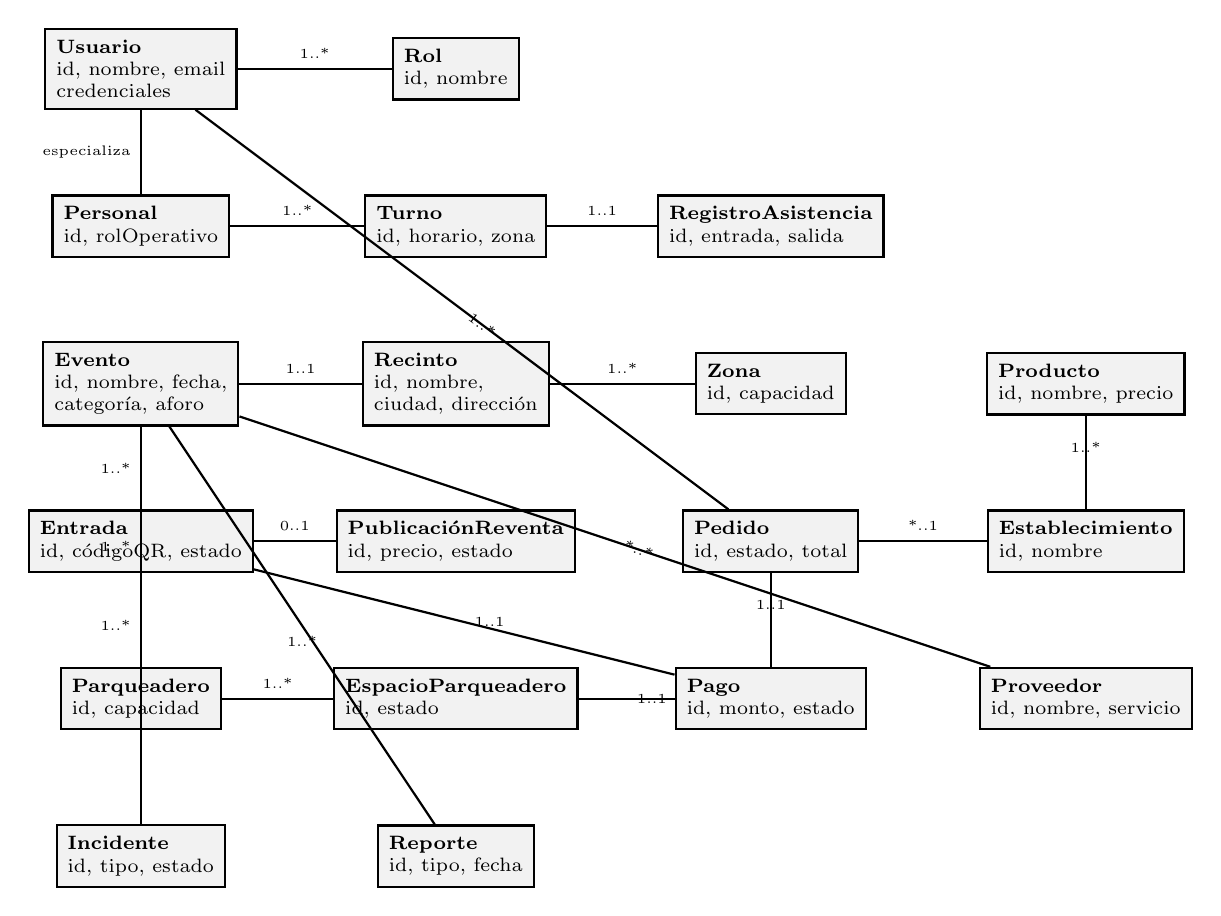
\begin{tikzpicture}[
  class/.style={draw, rectangle, align=left, font=\scriptsize, inner sep=4pt, fill=gris},
  >={Stealth[length=2mm]}, thick, every node/.style={font=\tiny}
]
\node[class] (usuario)         at (0,9)   {\textbf{Usuario}\\id, nombre, email\\credenciales};
\node[class] (rol)             at (4,9)   {\textbf{Rol}\\id, nombre};
\node[class] (personal)        at (0,7)   {\textbf{Personal}\\id, rolOperativo};
\node[class] (turno)           at (4,7)   {\textbf{Turno}\\id, horario, zona};
\node[class] (asistencia)      at (8,7)   {\textbf{RegistroAsistencia}\\id, entrada, salida};
\node[class] (evento)          at (0,5)   {\textbf{Evento}\\id, nombre, fecha,\\categoría, aforo};
\node[class] (recinto)         at (4,5)   {\textbf{Recinto}\\id, nombre,\\ciudad, dirección};
\node[class] (zona)            at (8,5)   {\textbf{Zona}\\id, capacidad};
\node[class] (entrada)         at (0,3)   {\textbf{Entrada}\\id, códigoQR, estado};
\node[class] (reventa)         at (4,3)   {\textbf{PublicaciónReventa}\\id, precio, estado};
\node[class] (pedido)          at (8,3)   {\textbf{Pedido}\\id, estado, total};
\node[class] (establecimiento) at (12,3)  {\textbf{Establecimiento}\\id, nombre};
\node[class] (producto)        at (12,5)  {\textbf{Producto}\\id, nombre, precio};
\node[class] (parqueadero)     at (0,1)   {\textbf{Parqueadero}\\id, capacidad};
\node[class] (espacio)         at (4,1)   {\textbf{EspacioParqueadero}\\id, estado};
\node[class] (pago)            at (8,1)   {\textbf{Pago}\\id, monto, estado};
\node[class] (proveedor)       at (12,1)  {\textbf{Proveedor}\\id, nombre, servicio};
\node[class] (incidente)       at (0,-1)  {\textbf{Incidente}\\id, tipo, estado};
\node[class] (reporte)         at (4,-1)  {\textbf{Reporte}\\id, tipo, fecha};

\draw (usuario) -- (rol)             node[midway, above] {1..*};
\draw (personal) -- (usuario)        node[midway, left]  {especializa};
\draw (personal) -- (turno)          node[midway, above] {1..*};
\draw (turno) -- (asistencia)        node[midway, above] {1..1};
\draw (evento) -- (entrada)          node[midway, left]  {1..*};
\draw (evento) -- (recinto)          node[midway, above] {1..1};
\draw (recinto) -- (zona)            node[midway, above] {1..*};
\draw (entrada) -- (reventa)         node[midway, above] {0..1};
\draw (evento) -- (parqueadero)      node[midway, left]  {1..*};
\draw (parqueadero) -- (espacio)     node[midway, above] {1..*};
\draw (usuario) -- (pedido)          node[midway, right, sloped] {1..*};
\draw (pedido) -- (establecimiento)  node[midway, above] {*..1};
\draw (establecimiento) -- (producto) node[midway, above] {1..*};
\draw (entrada) -- (pago)            node[midway, right] {1..1};
\draw (pedido) -- (pago)             node[midway, above] {1..1};
\draw (espacio) -- (pago)            node[midway, right] {1..1};
\draw (evento) -- (proveedor)        node[midway, right, sloped] {*..*};
\draw (evento) -- (incidente)        node[midway, left]  {1..*};
\draw (evento) -- (reporte)          node[midway, below] {1..*};
\end{tikzpicture}
\caption{Diagrama de clases UML — modelo de dominio (versión simplificada).}
\label{fig:dominio}
\end{figure}
\end{landscape}

% ==================== Stakeholders ====================
\section{Stakeholders e intereses}
\label{sec:stakeholders}

\begin{center}
\begin{longtable}{|p{3.6cm}|p{3.8cm}|p{6.9cm}|}
\hline
\textbf{Rol/Nombre} & \textbf{Información de Contacto} & \textbf{Intereses / expectativas} \\
\hline
\endhead
Cliente & Rol dentro del sistema (se autentica con su cuenta) & Comprar y revender entradas de
forma confiable, consultar sus pedidos y parqueadero, y recibir su QR sin fallas en el ingreso.\\
\hline
Organizador & Rol dentro del sistema & Crear y planificar eventos, asignar personal y
proveedores, y monitorear la operación en tiempo real.\\
\hline
Empleado / Personal operativo & Rol dentro del sistema & Consultar sus turnos y asignaciones,
solicitar cambios de turno y registrar su asistencia sin fricción.\\
\hline
Administrador & Rol dentro del sistema & Gestionar usuarios, roles, recintos y configuración
general con control de acceso auditable.\\
\hline
Supervisor de emergencia & Rol dentro del sistema & Activar y coordinar protocolos de evacuación
con información confiable y actualizada en tiempo real.\\
\hline
Proveedor externo & Gestionado por el organizador (módulo Proveedores) & Ser asignado
correctamente a los eventos que contrata y recibir la información logística necesaria.\\
\hline
Equipo Hexacore (Daniel Cristancho, Samuel Emperador, Sebastián Sánchez, Diego Coronado) &
\url{semperadorcontreras@gmail.com} (contacto del equipo) & Diseñar y sustentar una arquitectura que
satisfaga los atributos de calidad priorizados y cumpla los requisitos del curso.\\
\hline
Profesor / Evaluador del curso & Curso de Arquitectura de Software & Verificar que el SAD cumpla
la plantilla exigida y que las decisiones arquitectónicas estén justificadas.\\
\hline
\end{longtable}
\end{center}

% ==================== ASR ====================
\section{Requisitos Arquitectónicamente Significativos (ASR)}
\label{sec:asr}

La Tabla \ref{tab:asr} presenta el Árbol de Utilidad del proyecto: los escenarios de calidad que
tienen impacto arquitectónico real, derivados de los atributos priorizados en
\textit{ArchitecturalProposal.tex} y de los requisitos no funcionales de la sección
\ref{sec:rnf}. La columna \textbf{RNF} indica qué requisito verificable pone a prueba cada
escenario; entre los dos elementos hay una diferencia de propósito: el RNF fija el umbral
(\textit{cuánto}), el ASR describe la situación concreta que lo tensiona (\textit{cuándo y bajo
qué condiciones}).

Cada escenario se califica con el par \textbf{(Importancia, Dificultad)} en escala
Alta/Media/Baja, como pide el método del Árbol de Utilidad:

\begin{itemize}
  \item \textbf{Importancia}: qué tanto afecta al negocio que ese escenario \textit{no} se
  cumpla. Es la importancia \textit{del escenario}, que no siempre coincide con la prioridad
  global de su atributo --- por ejemplo, la Seguridad física está priorizada como Media en el
  conjunto del sistema, pero el escenario ASR-13 (fallar al notificar una evacuación) tiene
  importancia Alta porque compromete la integridad de las personas.
  \item \textbf{Dificultad}: qué tan difícil es técnicamente satisfacerlo con la arquitectura
  propuesta.
\end{itemize}

Los escenarios calificados \textbf{(Alta, Alta)} --- ASR-01, ASR-04 y ASR-13 --- son los que
concentran el riesgo arquitectónico del proyecto y, por lo tanto, los candidatos naturales a
respaldarse con una prueba de concepto medida en vez de solo con razonamiento.

\begin{landscape}
\begin{center}
\begin{longtable}{|p{1cm}|p{2.9cm}|p{2.1cm}|p{2.3cm}|p{1.7cm}|p{1.5cm}|p{6.1cm}|p{1.4cm}|p{1.4cm}|}
\caption{Árbol de Utilidad --- escenarios de calidad con su par (Importancia, Dificultad) y el
RNF que verifican.}\label{tab:asr}\\
\hline
\textbf{ID ASR} & \textbf{Título} & \textbf{Atributo} & \textbf{Sub-atributo} &
\textbf{CU(s)} & \textbf{RNF} & \textbf{Escenario} & \textbf{Impor-tancia} &
\textbf{Difi-cultad}\\
\hline
\endfirsthead
\multicolumn{9}{l}{\small\textit{Tabla \thetable{} --- continuación}}\\
\hline
\textbf{ID ASR} & \textbf{Título} & \textbf{Atributo} & \textbf{Sub-atributo} &
\textbf{CU(s)} & \textbf{RNF} & \textbf{Escenario} & \textbf{Impor-tancia} &
\textbf{Difi-cultad}\\
\hline
\endhead
\hline
\multicolumn{9}{r}{\small\textit{Continúa en la página siguiente\ldots}}\\
\endfoot
\hline
\endlastfoot
ASR-01 & Bloqueo de doble venta en reventa & Consistencia & Concurrencia de datos & CU-006 &
RNF-01, RNF-02 & Dos compradores intentan adquirir simultáneamente la misma entrada publicada en
reventa; el sistema garantiza que solo uno complete la compra y el otro reciba de inmediato un
mensaje de no disponibilidad. & Alta & Alta\\
\hline
ASR-02 & Disponibilidad durante el ingreso masivo & Disponibi-lidad & Tolerancia a fallos &
CU-002, CU-021, CU-022 & RNF-03, RNF-04 & Ante la caída de una instancia del servicio de
validación de QR durante el ingreso al recinto, el balanceador redirige el tráfico a instancias
sanas sin interrupción perceptible para el asistente. & Alta & Media\\
\hline
ASR-03 & Protección de datos de pago y credenciales & Seguridad & Confiden-cialidad & CU-001,
CU-024, CU-031 & RNF-05, RNF-06 & Un intento de acceso no autorizado a datos de pago o
credenciales es rechazado por el API Gateway y queda registrado para auditoría. & Alta &
Media\\
\hline
ASR-04 & Respuesta bajo carga en apertura de venta & Rendimiento & Tiempo de respuesta & CU-001,
CU-005 & RNF-07, RNF-08 & Durante la apertura de venta de un evento masivo, miles de usuarios
consultan disponibilidad y compran de forma simultánea; la mayoría de las solicitudes se resuelve
en tiempos cortos y estables. & Alta & Alta\\
\hline
ASR-05 & Actualización de aforo y zonas en tiempo real & Tiempo real & Actualización de estado &
CU-010, CU-019 & RNF-09 & El aforo y el estado de las zonas se reflejan en los tableros de
monitoreo con baja latencia tras el registro de un ingreso o un incidente. & Media & Alta\\
\hline
ASR-06 & Escalado independiente del servicio de Entradas & Escala-bilidad & Escala-bilidad
horizontal & CU-001, CU-006 & RNF-10 & Ante un incremento súbito de tráfico en el servicio de
Entradas durante una preventa, aumentan sus instancias sin afectar el rendimiento de los demás
dominios. & Media & Media\\
\hline
ASR-07 & Auditoría de transferencias y pagos & Traza-bilidad & Audita-bilidad & CU-006, CU-031 &
RNF-11 & Cada transferencia de entrada, pago o reembolso queda registrada con usuario, fecha y
resultado, consultable en un reporte de auditoría. & Media & Baja\\
\hline
ASR-08 & Interfaces especializadas por rol & Usabilidad & Adecuación a la tarea & Todos los CU
(por interfaz) & RNF-12 & Un usuario nuevo de cada rol completa su tarea principal en su interfaz
correspondiente sin capacitación previa. & Media & Baja\\
\hline
ASR-09 & Evolución independiente de dominios & Manteni-bilidad & Modifica-bilidad & Todos los CU
(por micro-servicio) & RNF-13 & Un cambio en las reglas de negocio de Parqueaderos se implementa y
despliega sin requerir cambios ni redespliegue del servicio de Entradas. & Media & Media\\
\hline
ASR-10 & Consumo uniforme vía API & Porta-bilidad & Independencia de plataforma & Todos los CU &
RNF-14 & Una misma funcionalidad de backend se consume igual desde el portal web y desde la app
móvil, sin duplicar lógica de negocio. & Media & Baja\\
\hline
ASR-11 & Sustitución del proveedor de pagos sin reescribir el dominio & Integra-bilidad &
Adaptación de interfaces & CU-001, CU-011, CU-024 & RNF-16 & La organización cambia de pasarela de
pagos por costos; el equipo reemplaza el adaptador de pagos y los servicios de Entradas,
Parqueaderos y Pedidos siguen funcionando sin modificar su lógica de negocio. & Media & Media\\
\hline
ASR-12 & Actualización de un servicio con el evento en curso & Desplega-bilidad & Despliegue sin
interrupción & Todos los CU (por micro-servicio) & RNF-15 & Se detecta un defecto en el servicio
de Pedidos durante un evento activo; se despliega la corrección sin detener la venta ni el ingreso
de asistentes, y con posibilidad de revertir si la versión nueva falla. & Media & Media\\
\hline
ASR-13 & Notificación garantizada de evacuación & Seguridad física (Safety) & Respuesta ante
emergencia & CU-010 & RNF-17 & El supervisor activa el protocolo de evacuación; todo el personal
en campo recibe su instrucción específica en segundos, incluso si el proveedor de notificaciones
responde con lentitud o una instancia del servicio falla. & Alta & Alta\\
\hline
ASR-14 & Prueba aislada de cada microservicio & Comproba-bilidad & Aislamiento de dependencias &
Todos los CU (por micro-servicio) & RNF-18 & Un integrante prueba la lógica de su dominio sin
levantar los otros cinco microservicios ni depender de la pasarela de pagos real, sustituyéndolos
por dobles de prueba. & Media & Baja\\
\end{longtable}
\end{center}
\end{landscape}

% ==================== Restricciones ====================
\section{Restricciones}
\label{sec:restricciones}

\begin{center}
\begin{longtable}{|p{3.2cm}|p{2.8cm}|p{7cm}|}
\hline
\textbf{Restricción} & \textbf{Categoría} & \textbf{Descripción} \\
\hline
\endhead
Arquitectura de microservicios con base de datos independiente por dominio & Técnica & Decisión
fundacional ya tomada por el equipo (ver ADR-01); cualquier solución a un ASR debe respetar esta
separación por dominio.\\
\hline
Soporte de picos de miles de usuarios concurrentes & Técnica & El sistema debe soportar la
concurrencia propia de la apertura de venta y el ingreso masivo al recinto sin degradar el
servicio.\\
\hline
Equipo de 4 integrantes, 8 CU por persona & Organizacional & La distribución de trabajo (Daniel
Cristancho, Samuel Emperador, Sebastián Sánchez, Diego Coronado) condiciona qué componentes
prototipa cada integrante para Entrega 1 y Entrega 2.\\
\hline
Documento basado en el estándar arc42 & Convencional & La plantilla y estructura de este
documento las exige el curso; no pueden omitirse secciones.\\
\hline
Fechas y formato de entrega del curso & Convencional & Entrega 1 (SAD v1) y Entrega 2 (prototipo +
SAD v2) deben respetar las fechas y reglas de entrega definidas por el curso.\\
\hline
\end{longtable}
\end{center}

% ==================== Contexto y alcance ====================
\section{Contexto y Alcance}
\label{sec:contexto}

El sistema interactúa con cinco roles de usuario (Cliente, Organizador, Empleado, Administrador y
Supervisor de emergencia) y dos sistemas externos (Pasarela de Pagos y Proveedor de
Notificaciones). La Figura \ref{fig:contexto} muestra el diagrama de contexto (Nivel 1 del modelo
C4).

\begin{figure}[H]
\centering
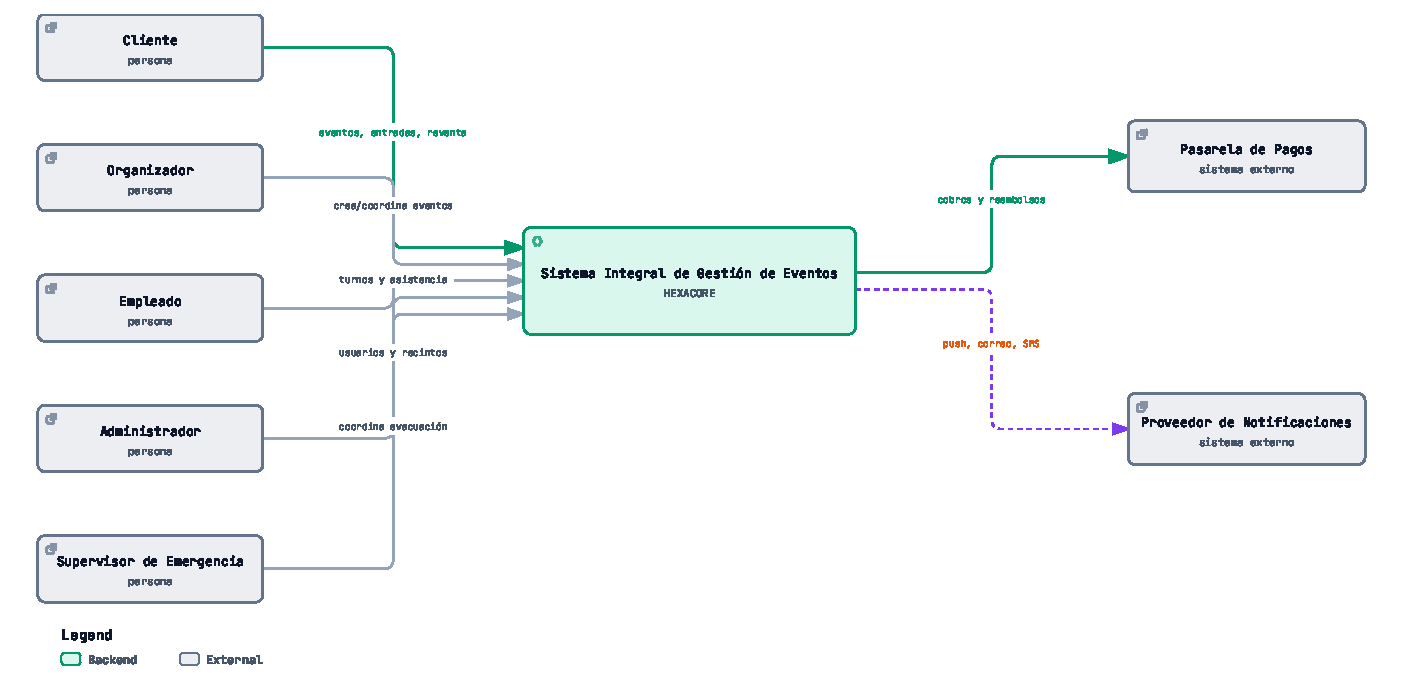
\includegraphics[width=\textwidth]{Diagrams/ArchifyPDF/01-contexto.pdf}
\caption{Diagrama de contexto (Nivel 1, modelo C4).}
\label{fig:contexto}
\end{figure}

\begin{center}
\begin{longtable}{p{3cm}p{3cm}p{6.5cm}}
\toprule
\textbf{Origen} & \textbf{Destino} & \textbf{Descripción}\\
\midrule
Cliente & Sistema & Consulta eventos, compra y revende entradas, reserva parqueadero.\\
Organizador & Sistema & Crea eventos, asigna personal y coordina la operación.\\
Empleado & Sistema & Consulta turnos y registra ingreso/salida.\\
Administrador & Sistema & Administra usuarios, personal y configuración.\\
Supervisor de emergencia & Sistema & Activa y coordina el protocolo de evacuación.\\
Sistema & Pasarela de Pagos & Procesa compras, reventas y reembolsos.\\
Sistema & Proveedor de Notificaciones & Envía notificaciones push, correo y SMS.\\
\bottomrule
\caption{Relaciones del diagrama de contexto.}
\end{longtable}
\end{center}

El diagrama de panorama de sistemas (\textit{System Landscape}, \textit{Diagrams/ArchifyPDF/04-panorama.pdf}
en \textit{C4Diagrams.tex}) amplía este alcance mostrando además cómo el sistema se relaciona con
otros sistemas de la organización (Contabilidad y Facturación, CRM/Marketing y una plataforma de
Analítica), fuera del alcance de este documento pero relevantes para entender el ecosistema
completo.

% ==================== Vista de contenedores ====================
\section{Vista de contenedores}
\label{sec:contenedores}

El sistema se divide en tres interfaces desplegables (Portal Web del Cliente, Portal Web
Administrativo/Operativo y App Móvil), todas consumiendo el mismo backend a través de un API
Gateway. La \textbf{App Móvil} está construida en \textbf{Flutter} (ADR-08), lo que permite generar
desde una sola base de código los binarios de Android e iOS, y sirve tanto al rol Cliente como al rol
Personal: el login identifica el rol del usuario autenticado y la navegación interna abre el conjunto
de pantallas correspondiente — no son dos apps distribuidas por separado (ver ADR-07). El backend está compuesto por microservicios independientes por dominio
(Entradas/Mercado Secundario, Personal, Eventos/Emergencias, Parqueaderos) y por infraestructura de
soporte (Redis, cola de mensajes y bases de datos por servicio). La Figura \ref{fig:contenedores}
presenta el diagrama de contenedores.

\begin{figure}[H]
\centering
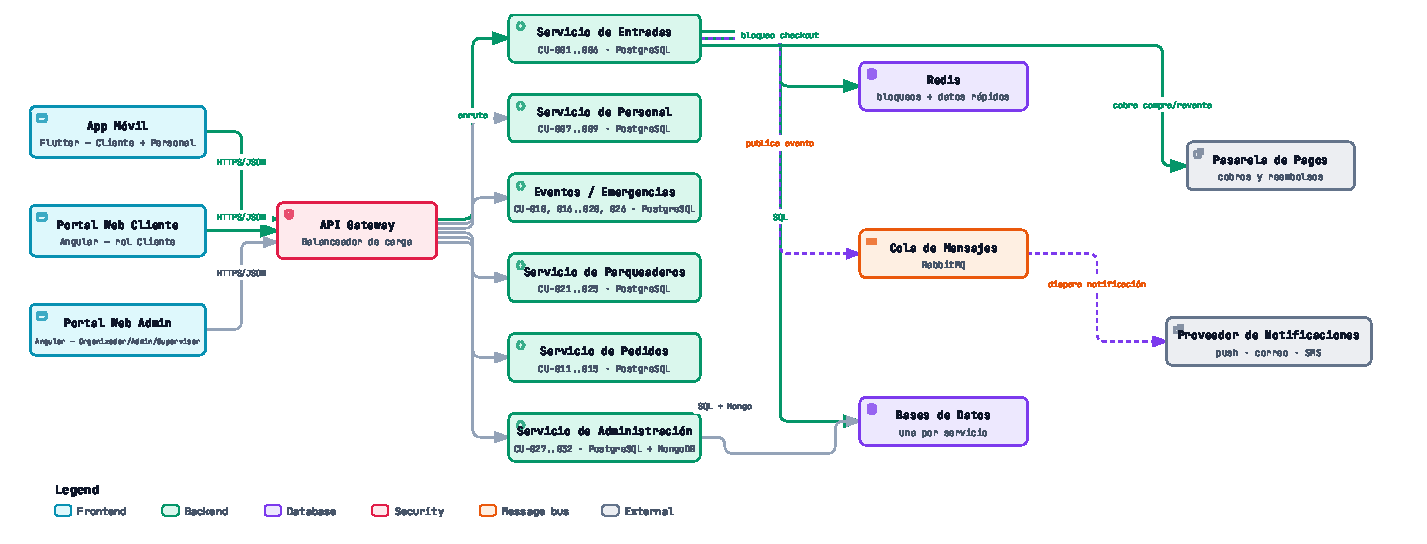
\includegraphics[width=\textwidth]{Diagrams/ArchifyPDF/02-contenedores.pdf}
\caption{Diagrama de contenedores (Nivel 2, modelo C4).}
\label{fig:contenedores}
\end{figure}


\begin{itemize}
\item \textbf{API Gateway + balanceador de carga:} punto único de entrada al backend; centraliza
autenticación, autorización, validación de tokens y enrutamiento hacia el microservicio
correspondiente.
\item \textbf{Microservicios:} Entradas/Mercado Secundario, Personal, Eventos/Emergencias y
Parqueaderos, cada uno con su propia base de datos para reducir el acoplamiento entre dominios.
\item \textbf{Redis:} bloqueo temporal de recursos en disputa (p. ej. una entrada en reventa
durante el checkout) y datos de acceso rápido (aforo, ocupación, sesiones).
\item \textbf{Cola de mensajes (RabbitMQ, ADR-10):} desacopla operaciones asíncronas: generación de
QR, notificaciones, auditoría, liquidación de pagos y alertas de emergencia.
\item \textbf{Servicios externos:} Pasarela de Pagos y Proveedor de Notificaciones, integrados vía
API y, en el caso de notificaciones, disparados de forma asíncrona desde la cola de mensajes.
\end{itemize}

% ==================== Vista de componentes ====================
\section{Vista de componentes}
\label{sec:componentes}

Se detalla primero el contenedor \textbf{Servicio de Entradas y Mercado Secundario}, por ser el
que resuelve el caso de uso complejo CU-006 (Gestión del Mercado Secundario de Entradas), y luego,
al mismo nivel de detalle, los otros tres microservicios de dominio. La Figura
\ref{fig:componentes} muestra los componentes internos del Servicio de Entradas.

\begin{figure}[H]
\centering
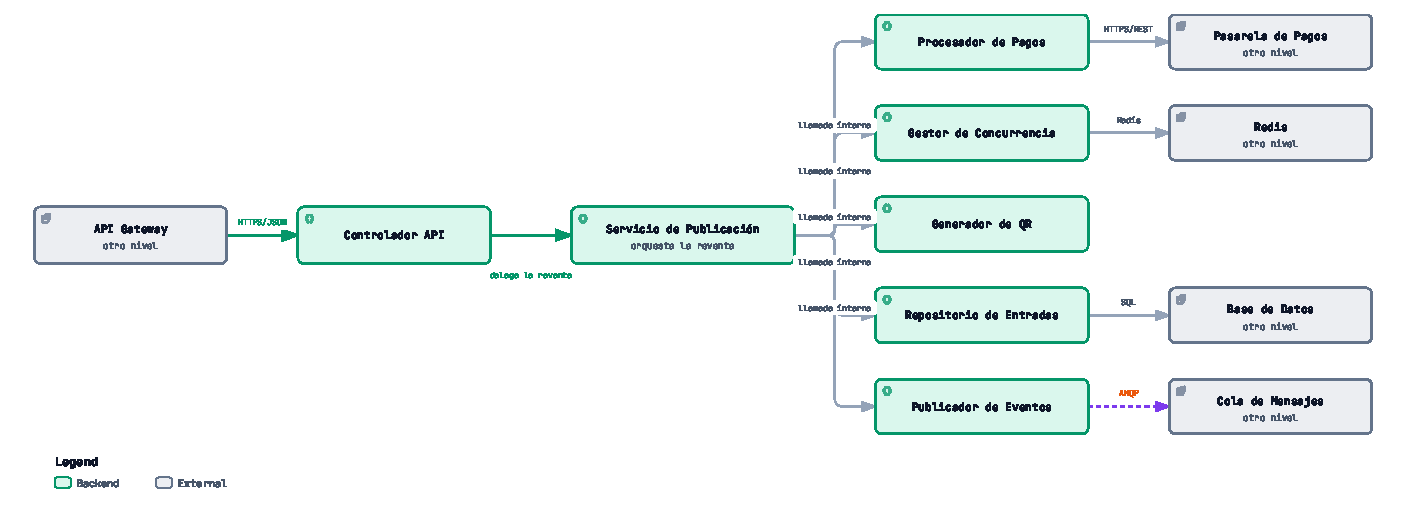
\includegraphics[width=\textwidth]{Diagrams/ArchifyPDF/03-componentes.pdf}
\caption{Diagrama de componentes — Servicio de Entradas y Mercado Secundario (Nivel 3, modelo
C4).}
\label{fig:componentes}
\end{figure}

El flujo interno es: el \textbf{Controlador API} recibe la solicitud enrutada por el API Gateway y
la delega al \textbf{Servicio de Publicación}, que orquesta la operación de reventa. Este componente
solicita al \textbf{Gestor de Concurrencia} el bloqueo temporal de la entrada en Redis, invoca al
\textbf{Procesador de Pagos} para cobrar la transacción contra la Pasarela de Pagos, usa el
\textbf{Generador de QR} para invalidar el código anterior y emitir uno nuevo, persiste el cambio
de propiedad mediante el \textbf{Repositorio de Entradas}, y finalmente notifica el resultado a
través del \textbf{Publicador de Eventos} hacia la cola de mensajes.

\subsection{Servicio de Personal}

El \textbf{Controlador API} enruta la solicitud hacia el \textbf{Servicio de Asignación de
Personal}, que valida rol, disponibilidad y horario del empleado con apoyo del \textbf{Validador
de Conflictos} antes de confirmar una asignación o un cambio de turno. El \textbf{Gestor de
Turnos} calcula horarios y, junto con el \textbf{Repositorio de Personal}, persiste asignaciones,
turnos y registros de asistencia. El \textbf{Publicador de Eventos} notifica, vía cola de
mensajes, la confirmación de asignaciones y cambios de turno al empleado y al supervisor.

\subsection{Servicio de Eventos / Emergencias}

El \textbf{Controlador API} enruta hacia el \textbf{Servicio de Gestión de Eventos} (CRUD de
eventos, localidades y aforo) o hacia el \textbf{Servicio de Protocolo de Emergencia}, según la
operación. Al activarse una evacuación, este último consulta al \textbf{Gestor de Zonas y Aforo}
(apoyado en Redis para datos de baja latencia) para identificar zonas afectadas, salidas y rutas
disponibles; persiste el incidente mediante el \textbf{Repositorio de Eventos}; y usa el
\textbf{Publicador de Eventos} para difundir alertas y actualizaciones de estado a través de la
cola de mensajes hacia el personal y los asistentes.

\subsection{Servicio de Parqueaderos}

El \textbf{Controlador API} delega en el \textbf{Servicio de Reservas}, que gestiona la reserva
previa y el ingreso/salida de vehículos. El \textbf{Gestor de Ocupación} mantiene en Redis el
estado de ocupación por zona en tiempo real. El \textbf{Procesador de Cobro} invoca la Pasarela de
Pagos para tarifas y reservas. El \textbf{Repositorio de Espacios} persiste las asignaciones, y el
\textbf{Publicador de Eventos} notifica confirmaciones hacia la cola de mensajes.

% ==================== Vista de procesos ====================
\section{Vista de procesos}
\label{sec:procesos}

Se documentan los dos procesos más críticos del sistema desde el punto de vista de los atributos
de calidad: la reventa de una entrada (concurrencia y consistencia) y la evacuación ante una
emergencia (disponibilidad y tiempo real).

\subsection{Reventa de una entrada (CU-006)}

La Figura \ref{fig:secuencia} muestra, con líneas de vida y mensajes numerados, cómo colaboran los
contenedores para resolver una compra en el mercado secundario.

\begin{figure}[H]
\centering
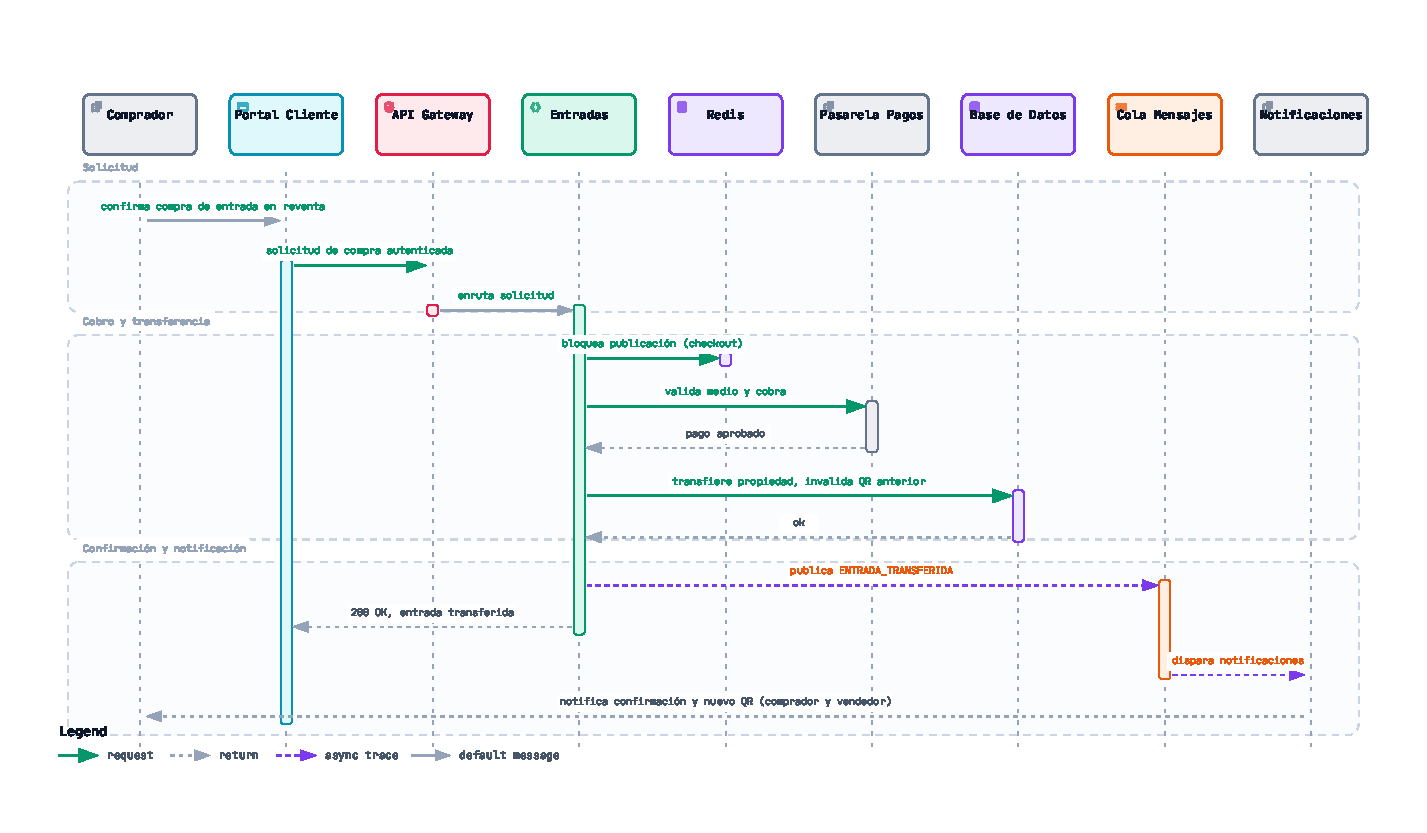
\includegraphics[width=\textwidth]{Diagrams/ArchifyPDF/05-secuencia.pdf}
\caption{Diagrama de secuencia — reventa de una entrada (CU-006).}
\label{fig:secuencia}
\end{figure}

\begin{enumerate}
\item El comprador confirma la compra de una entrada publicada en el mercado secundario.
\item El API Gateway enruta la solicitud autenticada hacia el Servicio de Entradas.
\item El Servicio de Entradas bloquea temporalmente la publicación en Redis, para impedir que otro
comprador la adquiera de forma simultánea.
\item Se valida el medio de pago y se cobra el valor de la entrada mediante la Pasarela de Pagos.
\item Se transfiere la propiedad de la entrada y se invalida el código QR anterior en la base de
datos.
\item Se publica el evento \texttt{ENTRADA\_TRANSFERIDA} en la cola de mensajes.
\item El Proveedor de Notificaciones envía la confirmación y el nuevo código QR al comprador y al
vendedor, de forma desacoplada del flujo principal.
\end{enumerate}

\subsection{Evacuación ante emergencias (CU-010)}

\begin{enumerate}
\item El supervisor activa el protocolo de evacuación desde el Portal Web Administrativo,
registrando el tipo y ubicación de la emergencia.
\item El servicio de Eventos/Emergencias identifica las zonas potencialmente afectadas y consulta
el aforo actual, las salidas disponibles y las rutas configuradas.
\item El sistema presenta las rutas y zonas recomendadas; el supervisor confirma el protocolo.
\item Se notifica al personal operativo y se envían instrucciones a los asistentes mediante la
cola de mensajes y el Proveedor de Notificaciones.
\item El sistema monitorea las zonas en tiempo real mientras el supervisor atiende alertas
(ruta bloqueada, zona congestionada, cambio de nivel de emergencia) hasta confirmar la
finalización.
\end{enumerate}

% ==================== Vista física ====================
\section{Vista física}
\label{sec:fisica}

La Figura \ref{fig:despliegue} muestra el ambiente de \textbf{producción}: los dispositivos del
usuario acceden vía CDN a los archivos estáticos y vía balanceador + API Gateway al backend, que
corre en un clúster de aplicación con réplicas por microservicio, respaldado por un clúster de
bases de datos, un clúster Redis y un clúster de mensajería.

\begin{figure}[H]
\centering
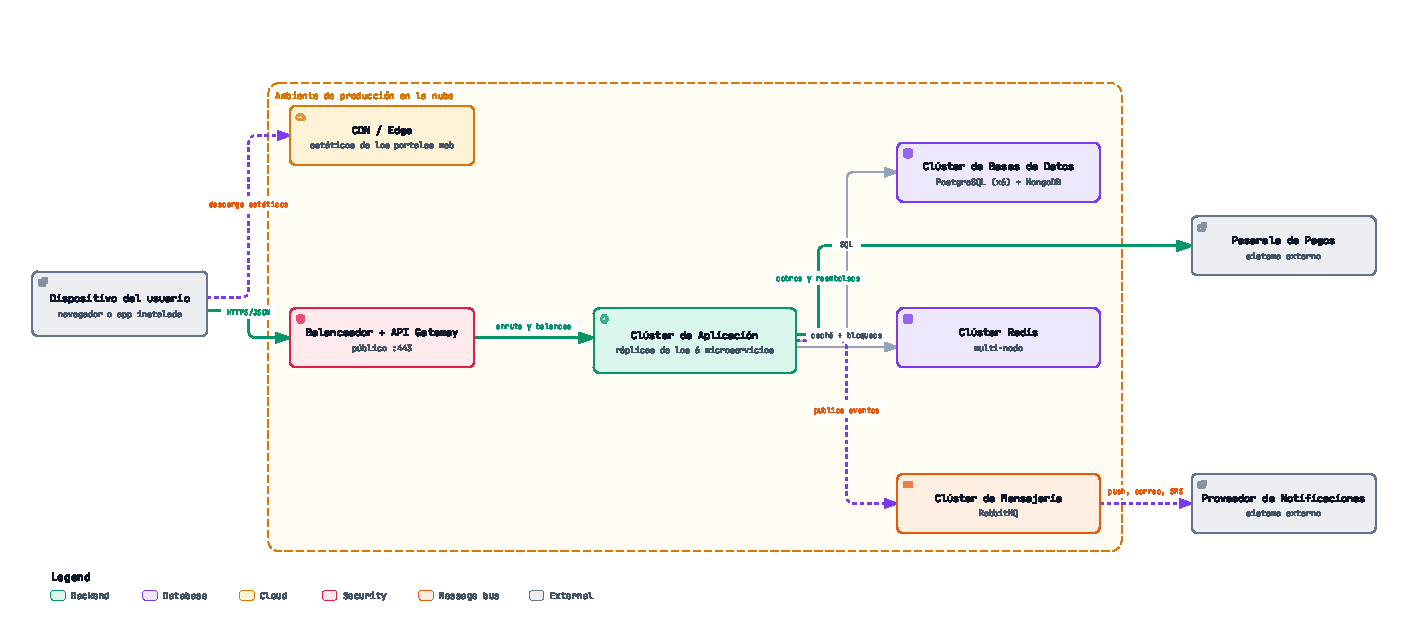
\includegraphics[width=\textwidth]{Diagrams/ArchifyPDF/06-despliegue.pdf}
\caption{Diagrama de despliegue — ambiente de producción (modelo C4).}
\label{fig:despliegue}
\end{figure}

Los ambientes de \textbf{desarrollo} y \textbf{pruebas} reutilizan la misma topología del
diagrama de despliegue de producción, a menor escala: una única réplica por microservicio (sin
balanceo horizontal), sin CDN (los archivos estáticos se sirven directamente desde el servidor de
aplicación), y con Redis, la cola de mensajes y las bases de datos desplegadas en un único nodo
compartido en vez de un clúster. El ambiente de \textbf{desarrollo} se despliega automáticamente
mediante integración continua ante cada cambio en la rama principal, con datos de prueba mínimos
para verificación funcional rápida. El ambiente de \textbf{pruebas} se usa para validación
funcional end-to-end y pruebas de carga previas a cada entrega, con datos sintéticos que simulan
la concurrencia esperada durante la apertura de venta y el ingreso masivo, de forma que los ASR de
disponibilidad y rendimiento (sección \ref{sec:asr}) puedan verificarse antes de producción. El
script de despliegue automatizado que provisiona ambos ambientes se entregará junto con el
prototipo funcional en la Entrega 2.

% ==================== Modelo de datos ====================
\section{Modelo de datos}
\label{sec:datos}

Siguiendo la decisión de una base de datos independiente por microservicio (ADR-01), cada dominio
tiene su propio esquema relacional. Las referencias entre dominios (p. ej. el propietario de una
\textit{Entrada} hacia \textit{Usuario}, que vive en el módulo de administración de cuentas) se
resuelven a nivel de aplicación mediante el identificador correspondiente, y no con llaves foráneas
físicas entre bases de datos distintas, lo cual es consistente con la separación de datos
establecida en ADR-01. A continuación se listan las entidades principales de cada esquema, con sus
llaves foráneas lógicas.

\subsection*{Esquema de Entradas / Mercado Secundario}
\begin{itemize}
\item \textbf{Entrada}(id, evento\_id, localidad\_id, propietario\_id, codigoQR, estado)
\item \textbf{PublicacionReventa}(id, entrada\_id, vendedor\_id, precio, estado)
\end{itemize}

\subsection*{Esquema de Personal}
\begin{itemize}
\item \textbf{Personal}(id, usuario\_id, rolOperativo)
\item \textbf{Turno}(id, personal\_id, evento\_id, zona\_id, horario)
\item \textbf{RegistroAsistencia}(id, turno\_id, horaEntrada, horaSalida)
\end{itemize}

\subsection*{Esquema de Eventos / Emergencias}
\begin{itemize}
\item \textbf{Evento}(id, nombre, fecha, categoria, recinto\_id, aforo)
\item \textbf{Recinto}(id, nombre, ciudad, direccion)
\item \textbf{Zona}(id, recinto\_id, capacidad)
\item \textbf{Incidente}(id, evento\_id, tipo, estado)
\end{itemize}

\subsection*{Esquema de Parqueaderos}
\begin{itemize}
\item \textbf{Parqueadero}(id, evento\_id, capacidad)
\item \textbf{EspacioParqueadero}(id, parqueadero\_id, estado)
\end{itemize}

\subsection*{Esquemas de administración general}
\begin{itemize}
\item \textbf{Usuario}(id, nombre, email, credenciales), \textbf{Rol}(id, nombre),
\textbf{UsuarioRol}(usuario\_id, rol\_id)
\item \textbf{Proveedor}(id, nombre, servicio)
\item \textbf{Pago}(id, tipo, monto, estado, referencia\_id, referencia\_tipo) — registra pagos de
Entradas, Pedidos o Parqueaderos mediante \texttt{referencia\_tipo}
\item \textbf{Pedido}(id, cliente\_id, establecimiento\_id, estado, total),
\textbf{Establecimiento}(id, nombre), \textbf{Producto}(id, establecimiento\_id, nombre, precio)
\item \textbf{Reporte}(id, tipo, fechaGeneracion)
\end{itemize}

El motor de base de datos concreto por dominio es \textbf{PostgreSQL} para los esquemas
transaccionales y \textbf{MongoDB} para Reportes (ADR-06).

% ==================== ADR ====================
\section{Registros de Decisiones Arquitectónicas (ADR)}
\label{sec:adr}

\subsection*{ADR-01 --- Arquitectura de microservicios por dominio}
\textbf{ASR relacionados:} ASR-06, ASR-09.\\
\textbf{Problema:} el sistema debe permitir que sus dominios (Entradas, Mercado Secundario,
Personal, Eventos, Parqueaderos, Emergencias) evolucionen y escalen de forma relativamente
independiente, sin que un cambio en uno arriesgue la disponibilidad de los demás.\\
\textbf{Solución:} se adopta una arquitectura de \textbf{microservicios}, uno por dominio, cada
uno con base de datos propia.\\
\textbf{Alternativa descartada:} monolito modular — dificulta escalar de forma independiente el
servicio de Entradas durante una apertura de venta sin sobre-aprovisionar los demás dominios.\\
\textbf{Consecuencias:} favorece mantenibilidad y escalabilidad independiente, a costa de mayor
complejidad operativa (más piezas de infraestructura) y de tener que gestionar consistencia
eventual entre servicios en vez de transacciones ACID únicas.

\subsection*{ADR-02 --- API Gateway y balanceador de carga}
\textbf{ASR relacionados:} ASR-02, ASR-03.\\
\textbf{Problema:} se necesita un punto único, seguro y disponible de entrada al backend para las
tres interfaces del sistema.\\
\textbf{Solución:} un \textbf{API Gateway} centraliza autenticación, autorización y enrutamiento;
un \textbf{balanceador de carga} distribuye solicitudes entre múltiples instancias de cada
microservicio.\\
\textbf{Alternativa descartada:} exponer cada microservicio directamente a los clientes — se
descartó por duplicar lógica de seguridad en cada interfaz y complicar el enrutamiento.\\
\textbf{Consecuencias:} centraliza seguridad y facilita el enrutamiento, pero introduce un
componente crítico que debe replicarse (mitigado con múltiples instancias detrás del
balanceador) para no convertirse en un punto único de falla.

\subsection*{ADR-03 --- Redis para bloqueo temporal y datos de acceso rápido}
\textbf{ASR relacionados:} ASR-01, ASR-05.\\
\textbf{Problema:} evitar que dos compradores completen simultáneamente la compra de la misma
entrada en reventa, y disponer de datos de aforo/ocupación con baja latencia.\\
\textbf{Solución:} \textbf{Redis} se usa como bloqueo distribuido temporal durante el checkout de
una reventa, y como caché de datos de acceso rápido (aforo, ocupación, sesiones).\\
\textbf{Alternativa descartada:} bloqueo pesimista directamente en la base de datos relacional —
se descartó por convertirse en cuello de botella bajo la carga concurrente esperada.\\
\textbf{Consecuencias:} resuelve la doble venta y acelera consultas frecuentes, pero añade un
punto adicional de falla que requiere su propia estrategia de disponibilidad (réplica/clúster).

\subsection*{ADR-04 --- Cola de mensajes para operaciones asíncronas}
\textbf{Estado:} \textit{completado por ADR-10} --- la decisión de usar una cola sigue vigente; el
motor concreto, que aquí quedó abierto como ``RabbitMQ/Kafka'', se cerró en ADR-10 con evidencia
medida.\\
\textbf{ASR relacionados:} ASR-04, ASR-07.\\
\textbf{Problema:} operaciones como notificaciones o liquidación de pagos no deben bloquear ni
hacer fallar la operación principal (compra, transferencia) cuando un servicio externo es lento o
falla temporalmente.\\
\textbf{Solución:} una \textbf{cola de mensajes (RabbitMQ/Kafka)} desacopla la generación de QR,
las notificaciones, la auditoría y la liquidación de pagos del flujo síncrono principal.\\
\textbf{Alternativa descartada:} comunicación síncrona directa con los servicios externos — se
descartó porque un fallo temporal del proveedor de notificaciones no debe bloquear la operación
principal.\\
\textbf{Consecuencias:} tolera fallos externos y mejora el rendimiento percibido, a costa de
consistencia eventual y de requerir monitoreo propio de las colas.

\subsection*{ADR-05 --- Stack de frontend por tipo de interfaz}
\textbf{Estado:} \textit{parcialmente superado por ADR-08} --- lo relativo a los portales web sigue
vigente; la decisión sobre el stack de la app móvil fue revertida el 2026-09-07. Se conserva el
texto original como registro de por qué se decidió así en su momento.\\
\textbf{ASR relacionados:} ASR-08, ASR-10, ASR-05.\\
\textbf{Problema:} las tres interfaces (portal web del cliente, portal web administrativo/operativo,
app móvil) deben implementarse en un lenguaje/framework concreto, sin comprometer el consumo
uniforme del backend vía API Gateway (ASR-10) ni la especialización por rol de cada interfaz
(ASR-08).\\
\textbf{Solución:} los portales web se construyen en \textbf{Angular + TypeScript} — su estructura de
módulos, \textit{guards} e \textit{interceptors} favorece el trabajo en paralelo de varios
integrantes con convenciones consistentes, y RxJS encaja con las actualizaciones en tiempo real de
ASR-05. La app móvil se construye en \textbf{Kotlin nativo sobre Android Studio} (Jetpack
Compose para la interfaz, \textit{coroutines}/\textit{Flow} para tiempo real), aprovechando que el
equipo ya domina ambos lenguajes; sirve a los roles Cliente y Personal desde un mismo proyecto
(ver ADR-07), por lo que ASR-08 se resuelve con navegación condicionada por rol en vez de con
binarios separados.\\
\textbf{Alternativa descartada:} un framework híbrido/\textit{cross-platform} (p. ej. React Native o
Flutter) para compartir código de interfaz entre web y móvil — se descartó porque ASR-10 ya evita
duplicar lógica de negocio en el cliente (esta vive en el backend, detrás del API Gateway), por lo
que compartir código de UI entre plataformas no aporta un beneficio arquitectónico claro frente al
costo de una capa de abstracción adicional y a la experiencia ya existente del equipo con Angular y
Kotlin nativos.\\
\textbf{Consecuencias:} cada interfaz evoluciona con las herramientas nativas de su plataforma sin
las limitaciones de un framework híbrido, a costa de mantener dos ecosistemas de \textit{build}/
pruebas distintos (TypeScript/npm y Kotlin/Gradle) y de no compartir código de UI entre web y móvil
— los contratos comunes quedan limitados a la especificación de la API (ver \texttt{App/shared/}).

\subsection*{ADR-06 --- Motor de base de datos por dominio (\textit{polyglot persistence})}
\textbf{ASR relacionados:} ASR-01, ASR-07.\\
\textbf{Problema:} ADR-01 estableció una base de datos propia por microservicio, pero dejó abierto
el motor concreto; los esquemas transaccionales (Entradas, Personal, Eventos/Emergencias,
Parqueaderos, cuentas/proveedores/pagos) tienen necesidades de consistencia distintas a las de
Reportes/analítica, cuyos datos son más variables y semi-estructurados.\\
\textbf{Solución:} \textbf{PostgreSQL} como motor relacional para todos los esquemas transaccionales
(uno por microservicio, ADR-01), y \textbf{MongoDB} como motor documental exclusivamente para el
esquema de Reportes dentro del servicio de administración.\\
\textbf{Alternativa descartada:} un único motor relacional (PostgreSQL) también para Reportes — se
descartó para no forzar un esquema rígido sobre datos de reportes cuya estructura varía entre tipos
de reporte, tal como ya anticipaba la sección de modelo de datos.\\
\textbf{Consecuencias:} cada esquema usa el motor más adecuado a su naturaleza (ACID para lo
transaccional, esquema flexible para reportes), a costa de operar y respaldar dos motores de base de
datos distintos en vez de uno solo.

\subsection*{ADR-07 --- App móvil unificada para Cliente y Personal}
\textbf{ASR relacionados:} ASR-08, ASR-10.\\
\textbf{Problema:} el diseño original (v1.1) proponía dos apps móviles nativas independientes, una
por rol (Cliente y Personal). Al construir el prototipo de la Entrega 2 con un equipo pequeño, mantener
dos proyectos Android desde cero duplica configuración de Gradle, tema visual y esqueleto de
navegación sin que exista todavía una razón operativa concreta (distribución, permisos de
dispositivo, política de actualización) que obligue a separarlos en esta etapa.\\
\textbf{Solución:} una única app (\texttt{App/frontend/app-movil}) con una pantalla de login
compartida. Las credenciales identifican el rol del usuario autenticado y la navegación interna abre
el conjunto de pantallas del rol correspondiente: Inicio/Entradas/Parqueadero/Pedidos para Cliente,
Turnos/Asistencia/Validación para Personal. Esta decisión sigue vigente tras el cambio de stack de
ADR-08: la app Flutter mantiene el mismo esquema de una sola app para ambos roles.\\
\textbf{Alternativa descartada:} mantener \textbf{App Móvil del Cliente} y \textbf{App Móvil del
Personal} como dos módulos/APKs independientes (diseño de la v1.1) — se descartó para este
prototipo porque el beneficio principal de separarlas (aislar del binario público de clientes las
pantallas y permisos operativos del personal, y poder distribuirlas y versionarlas por canales
distintos — tiendas públicas vs. MDM interno) todavía no tiene un requisito concreto que lo exija, y
el costo de mantener dos proyectos no se justifica en esta fase.\\
\textbf{Consecuencias:} menos código y configuración duplicados mientras el equipo es pequeño, y un
único punto de login para ambos roles. A cambio, el binario que instala un cliente cualquiera desde
la tienda pública contiene también las pantallas y — potencialmente — los permisos operativos del
personal (aunque inaccesibles sin credenciales válidas), lo que amplía la superficie de la app frente
a la alternativa separada; y ambos roles quedan acoplados a un mismo ciclo de release. Si el rol
Personal termina necesitando permisos de dispositivo, distribución o cadencia de actualización
distintos a los del Cliente, esta decisión debe revisarse y volver a separar los binarios.

\subsection*{ADR-08 --- Migración de la app móvil a Flutter}
\textbf{ASR relacionados:} ASR-08, ASR-09, ASR-10.\\
\textbf{Problema:} ADR-05 fijó \textbf{Kotlin nativo} para la app móvil y descartó explícitamente los
frameworks \textit{cross-platform}, con el argumento de que compartir código de interfaz no aportaba
un beneficio arquitectónico claro. Ese razonamiento omitió un requisito que sí es del proyecto: la
app debe llegar a \textbf{Android y iOS}. Con el stack nativo, cubrir iOS obliga a escribir y
mantener una segunda implementación completa (Swift/SwiftUI) de las mismas pantallas, lo que para un
equipo de cuatro personas duplica el esfuerzo de toda evolución de la interfaz y multiplica el riesgo
de que ambas plataformas se desincronicen.\\
\textbf{Solución:} la app móvil se reimplementa en \textbf{Flutter} (Dart), reemplazando la versión
Kotlin/Jetpack Compose. Una sola base de código produce los binarios de Android e iOS, conservando el
esquema de ADR-07 (una sola app para los roles Cliente y Personal, con el rol resuelto en el login).
La implementación incluye un cliente de API centralizado (\texttt{lib/services/api\_client.dart}) que
concentra el consumo del backend, de modo que la futura integración con el API Gateway quede en un
solo punto y no disperso por las pantallas (ASR-10).\\
\textbf{Alternativas consideradas:}
\begin{itemize}
  \item \textbf{Mantener Kotlin y añadir una app iOS nativa en Swift/SwiftUI} --- máxima fidelidad al
  look-and-feel de cada plataforma y acceso inmediato a APIs nuevas del sistema operativo, pero
  duplica la base de código de interfaz y el esfuerzo de mantenimiento (Modificabilidad, ASR-09).
  \item \textbf{Kotlin Multiplatform (KMM)} --- comparte la lógica de negocio y de red pero mantiene
  la interfaz nativa por plataforma; es el término medio, y se descartó porque el grueso del trabajo
  de este prototipo está justamente en la interfaz, que KMM no comparte.
  \item \textbf{Flutter} (elegida) --- una sola base de código para interfaz y lógica en ambas
  plataformas.
\end{itemize}
\textbf{Consecuencias:} una sola base de código para Android e iOS, y un único ciclo de build y
pruebas para la app móvil, a costa de: (1) renunciar a los widgets nativos reales --- Flutter dibuja
su propia interfaz con su motor de render, de modo que la fidelidad con cada plataforma es una
aproximación, no el control nativo; (2) sumar un tercer ecosistema de herramientas (Dart/pub) al del
web (TypeScript/npm) y el del backend; y (3) una curva de aprendizaje en Dart para el equipo. La
implementación Kotlin previa se elimina del repositorio; queda en el historial de Git si hiciera falta
recuperarla.\\
\textbf{Nota sobre la evidencia:} esta decisión se tomó reimplementando la app completa en Flutter y
comparándola con la versión Kotlin ya existente, no solo con un análisis en papel. La comparación
sistemática de métricas entre ambas implementaciones (tiempo de desarrollo, líneas de código,
arranque en frío, fidelidad visual) queda pendiente de documentarse como evidencia formal para la
Entrega 1.

\subsection*{ADR-09 --- Lenguaje y framework del backend}
\textbf{ASR relacionados:} ASR-04, ASR-06, ASR-09, ASR-14.\\
\textbf{Problema:} \texttt{App/services/*} estaba marcado como ``lenguaje por definir''. Es la única
decisión que bloquea empezar a codificar los seis microservicios, y debía tomarse con evidencia
medida --- no por preferencia ni por popularidad.\\
\textbf{Solución:} los microservicios de dominio se implementan en \textbf{NestJS} (Node.js +
TypeScript).\\
\textbf{Alternativas consideradas:} \textbf{NestJS} y \textbf{Spring Boot} (Java 17) se compararon
construyendo el mismo endpoint en ambos y midiéndolos bajo carga (PoC-04, ver
\texttt{App/PoCs/poc-04-lenguaje-backend/}). Se descartaron sin PoC: \textbf{Go}, porque nadie en el
equipo lo conoce y sumar un lenguaje nuevo con la entrega encima es el mayor riesgo de cronograma; y
\textbf{Python/FastAPI}, por su tipado opcional, poco conveniente con seis servicios desarrollados en
paralelo por cuatro personas.\\
\textbf{Evidencia (PoC-04):} mismo endpoint, misma respuesta byte por byte, 100 conexiones
concurrentes, 15 s por medición, cero errores:

\begin{center}
\begin{tabular}{llrrrr}
\toprule
\textbf{Candidato} & \textbf{Escenario} & \textbf{req/s} & \textbf{p50 (ms)} & \textbf{p97,5 (ms)} &
\textbf{RSS (MB)}\\
\midrule
NestJS & sin I/O & 21.071 & 4 & 5 & 156\\
NestJS & con 2 ms de I/O & 18.530 & 5 & 6 & 158\\
Spring Boot & sin I/O & 91.441 & 0 & 1 & 335\\
Spring Boot & con 2 ms de I/O & 32.288 & 3 & 4 & 337\\
\bottomrule
\end{tabular}
\end{center}

Arranque hasta la primera respuesta: \textbf{NestJS 0,28 s} frente a \textbf{Spring Boot 1,09 s}.

Tres lecturas de esos números:
\begin{enumerate}
  \item \textbf{Ambos cumplen RNF-07 con un margen enorme.} El umbral es p95 $\leq$ 500 ms y el peor
  caso medido fue 7 ms: setenta veces por debajo. El rendimiento, por lo tanto, \textbf{no es el
  criterio que decide} esta elección --- ninguno de los dos está cerca de incumplirlo.
  \item \textbf{Spring Boot rinde más, y conviene decirlo sin matizarlo:} 4,3$\times$ sin I/O. Pero la
  ventaja cae a 1,7$\times$ al añadir 2 ms de I/O simulada, y contra una base de datos real (5--20 ms)
  se encogería más. Cuanto más se parece el escenario a producción, menos pesa la diferencia.
  \item \textbf{NestJS arranca 4$\times$ más rápido y usa menos de la mitad de memoria}, lo que
  favorece a RNF-15 (despliegue sin interrupción) y al escalado elástico de ASR-06.
\end{enumerate}

\textbf{Por qué se elige NestJS pese a que Spring Boot rinde más:} porque el rendimiento ya está
resuelto por ambos con setenta veces de margen, y los criterios que sí quedan abiertos favorecen a
NestJS. En \textbf{Modificabilidad} (ASR-09) y \textbf{Comprobabilidad} (ASR-14, RNF-18), NestJS
impone módulos e inyección de dependencias --- el mismo modelo que el equipo ya aplica en los
portales Angular, y el que hace que sustituir dependencias externas por dobles de prueba sea directo.
Y el riesgo real del proyecto no es la latencia sino el cronograma: cuatro personas deben entregar
seis microservicios, y usar el lenguaje que ya escriben en el frontend elimina un cambio de contexto
completo.\\
\textbf{Consecuencias:} un solo lenguaje entre los portales web y el backend, con contratos de API que
pueden generar tipos para ambos lados (\texttt{App/shared/}). A cambio se acepta un techo de
rendimiento más bajo que el de Spring Boot --- irrelevante frente a los umbrales actuales, pero que
debería reevaluarse si algún servicio pasa a ser intensivo en CPU (los reportes con Map-Reduce, hoy
delegados a MongoDB, son el candidato a vigilar). Node ejecuta en un solo hilo por proceso, de modo
que el escalado es horizontal por réplicas, que es justamente lo que establecen ADR-01 y ASR-06.\\
\textbf{Validez de la evidencia:} el PoC mide un endpoint sin base de datos real, con cliente y
servidor en la misma máquina, y no llegó a los 2.000 usuarios concurrentes de RNF-07 (con 100
conexiones el generador de carga ya era el cuello de botella). Tampoco mide lo que probablemente más
pesa en la práctica: la velocidad de desarrollo del equipo. \textbf{Si alguno de los integrantes
tuviera experiencia sólida en Java}, esta decisión sería genuinamente discutible y Spring Boot
quedaría bien defendido por los datos.

\subsection*{ADR-10 --- Motor de la cola de mensajes: RabbitMQ}
\textbf{ASR relacionados:} ASR-04, ASR-07, ASR-13.\\
\textbf{Problema:} ADR-04 estableció que hace falta una cola de mensajes, pero dejó el motor sin
decidir, escrito como ``RabbitMQ/Kafka'' --- como si fueran intercambiables. No lo son: responden a
modelos distintos (cola de tareas frente a registro de eventos) y la elección condiciona cómo se
escriben los consumidores en los seis microservicios.\\
\textbf{Solución:} \textbf{RabbitMQ}.\\
\textbf{Evidencia (PoC-05, \texttt{App/PoCs/poc-05-cola-mensajes/}):} se publicó y consumió el evento
real \texttt{ENTRADA\_TRANSFERIDA} en ambos brokers (los dos en Docker, 500 mensajes por
combinación), midiendo la latencia de extremo a extremo:

\begin{center}
\begin{tabular}{llrrr}
\toprule
\textbf{Broker} & \textbf{Modo} & \textbf{p50 (ms)} & \textbf{p95 (ms)} & \textbf{msg/s}\\
\midrule
RabbitMQ & rápido (sin persistir) & \textbf{16,3} & \textbf{17,5} & 18.932\\
Kafka & rápido (\texttt{acks=0}) & 32,1 & 36,0 & 12.418\\
RabbitMQ & duradero (confirmado) & 162,0 & 282,1 & 1.619\\
Kafka & duradero (\texttt{acks=all}) & \textbf{31,6} & \textbf{57,9} & 7.702\\
\bottomrule
\end{tabular}
\end{center}

\textbf{El ganador se invierte según el modo}, y conviene decirlo sin matizarlo: sin durabilidad
RabbitMQ es el doble de rápido, pero \textbf{con durabilidad Kafka es cinco veces mejor} (31,6 ms
frente a 162 ms de mediana). La razón es estructural: RabbitMQ hace \texttt{fsync} por mensaje al
persistir y su latencia se multiplica por diez, mientras que Kafka escribe a un log secuencial y la
durabilidad le sale prácticamente gratis. Y el modo que importa aquí es el duradero: ni una
transferencia de entrada ni una alerta de evacuación pueden perderse porque el broker se reinició.

Sin embargo, \textbf{ambos cumplen RNF-17 con enorme margen}: el umbral es 10 s y el peor caso medido
—RabbitMQ duradero, p95— fue \textbf{282 ms}, treinta y cinco veces por debajo. Igual que en ADR-09,
la latencia no es el criterio que decide.

Se midió entonces lo que sí queda abierto, con el mismo escenario en ambos (10 eventos, 3 rechazados
a propósito):

\begin{center}
\begin{tabular}{lll}
\toprule
 & \textbf{RabbitMQ} & \textbf{Kafka}\\
\midrule
Cola de mensajes muertos (DLQ) & nativa, 5 líneas declarativas & no existe: hay que construirla\\
Imagen / memoria en reposo & 275 MB / 147 MB & 634 MB / 309 MB\\
Líneas para levantarlo & 9 & 15\\
Consola de administración & incluida & no incluida\\
Conceptos a dominar & colas, \textit{exchanges}, \textit{bindings} & + particiones, offsets, \textit{consumer groups}, retención\\
\bottomrule
\end{tabular}
\end{center}

\textbf{Por qué RabbitMQ pese a que Kafka es más rápido en modo duradero:} porque el uso que este
sistema le da a la cola es el de una \textbf{cola de tareas} —disparar una notificación, generar un
QR, registrar una auditoría, avisar de una evacuación— y no el de un \textit{registro de eventos}
con reproducción histórica y múltiples consumidores independientes, que es donde Kafka se justifica.
Para ese uso, RabbitMQ ofrece de fábrica lo que aquí sí hace falta: \textbf{DLQ y reintentos
nativos}, que ASR-07 y ASR-13 exigen para no perder en silencio un evento que falló. En Kafka eso
hay que construirlo y mantenerlo a mano. A eso se suma la mitad de memoria, la mitad de
configuración y una consola incluida, con un equipo de cuatro personas que además debe operar
PostgreSQL, MongoDB y Redis.\\
\textbf{Consecuencias:} se acepta una latencia mayor en modo duradero (282 ms de p95 frente a los
58 ms de Kafka) --- irrelevante frente al umbral de 10 s de RNF-17 --- y un techo de throughput más
bajo (1.619 msg/s duraderos). Ese techo es holgado para el volumen del sistema: los eventos se
generan por transferencia, pedido o alerta, no de forma continua. \textbf{Cuándo habría que
revisar esta decisión:} si aparece la necesidad de reproducir el histórico de eventos, de que varios
consumidores independientes lean el mismo flujo, o si el volumen se acerca al millar de mensajes por
segundo sostenido. En cualquiera de esos casos Kafka pasa a estar mejor justificado, y los números de
este PoC lo respaldarían.\\
\textbf{Validez de la evidencia:} un solo nodo de cada broker (en producción irían replicados, y ahí
Kafka replica mejor), todo en la misma máquina sin red de por medio, y 500 mensajes por medición ---
no se probó el comportamiento con colas de millones de mensajes, que es donde Kafka se separa de
verdad. Tampoco se midió la recuperación ante caída del broker, que es justamente el escenario que
motiva el modo duradero.


\subsection*{ADR-11 --- Autenticación entre servicios: RS256 y dos tokens}

\textbf{Contexto:} RNF-06 exige que \textit{toda} petición a un microservicio llegue autenticada y
autorizada por rol. Con seis dominios independientes (ADR-01), la pregunta es quién valida la sesión
y con qué. El CU-027 añade dos exigencias propias: que cerrar sesión surta efecto de verdad --- un
JWT es válido hasta que expira, lo firme quien lo firme --- y que la sesión no se caiga sola mientras
la persona está usando la aplicación.

\textbf{Alternativas consideradas:}
\begin{itemize}
  \item \textbf{HS256 con un secreto compartido.} Fue la primera implementación. Funciona mientras
        un solo servicio verifica, pero con HS256 firmar y verificar usan la misma clave: cada
        servicio que valida tokens podría \textbf{fabricar uno de administrador}. Con seis
        microservicios, seis lugares por donde se filtra la llave maestra.
  \item \textbf{Consultar al servicio de Administración en cada petición.} Autorización siempre
        exacta, pero convierte a ese servicio en un punto único de fallo para todo el sistema y le
        suma una llamada de red a cada operación.
  \item \textbf{RS256 con clave asimétrica} --- la elegida.
\end{itemize}

\textbf{Decisión:} tokens JWT firmados con \textbf{RS256}. La clave \textbf{privada} la tiene solo
el servicio de Administración, que es el único que emite; los demás reciben la \textbf{pública}, que
sirve para verificar y no para firmar. Al arrancar se comprueba que las dos claves se correspondan,
que sean RSA de 2048 bits o más y que en producción no sean las de desarrollo del repositorio.

Dos decisiones acompañan a la principal:

\begin{itemize}
  \item \textbf{Revocación por Redis (ADR-03).} Cada sesión cerrada se publica como
        \texttt{sesion-revocada:<jti>} con una vida igual a lo que le quedaba al token. Así los
        demás servicios rechazan un token revocado sin preguntar a Administración, y la lista no
        crece: cuando la clave expira, el token ya no valía por sí solo.
  \item \textbf{Dos tokens.} Uno de \textbf{acceso} de 15 minutos, que viaja en cada petición, y uno
        de \textbf{renovación} de 30 días sin uso, que solo viaja al renovar. Cada renovación emite
        uno nuevo e invalida el anterior; reutilizar uno gastado cierra la sesión entera, porque
        significa que dos partes tienen copia. En el navegador el token de renovación va en una
        cookie \texttt{HttpOnly; SameSite=Strict}, fuera del alcance de cualquier script inyectado.
\end{itemize}

\textbf{Atributo de calidad:} Seguridad (ASR-03) como motivación principal; Disponibilidad (ASR-02),
porque validar sin consultar evita el punto único de fallo; y Usabilidad (ASR-08), porque los dos
tokens evitan que la sesión se cierre sola con la aplicación abierta.

\textbf{Evidencia:} implementado y probado sobre el sistema real. Las pruebas de
\texttt{App/services/*/pruebas/} comprueban que un token con \texttt{alg: none} o firmado con la
clave pública como secreto HMAC se rechaza; que una sesión cerrada deja de valer \textit{en el otro
microservicio}; y que reutilizar un token de renovación ya gastado cierra la sesión. El API Gateway
(ADR-02) valida por subpetición contra \texttt{/sesiones/verificar}, y una prueba de defensa en
profundidad confirma que llamar directo a un servicio con la cabecera de identidad falsificada
devuelve 401.

\textbf{Consecuencias:} firmar con RSA cuesta más CPU que con HMAC, y cada petición protegida añade
una subpetición interna del gateway. A cambio, ningún servicio distinto del emisor puede fabricar un
token. \textbf{Cuándo revisar:} si el coste de la subpetición se notara bajo carga, los servicios
pueden verificar la firma por su cuenta con la clave pública y consultar Redis directamente ---
sigue sin necesitar la privada.

% ==================== Tácticas arquitectónicas ====================
\section{Tácticas arquitectónicas por atributo de calidad}
\label{sec:tacticas}

Las decisiones de la sección \ref{sec:adr} dicen \textit{qué} se eligió; esta sección dice
\textbf{cómo se realiza} cada atributo priorizado en el código, con el nombre de la táctica, el
mecanismo concreto que la implementa y la medición que la respalda. Cubre los cinco atributos
que la entrega exige demostrar en vivo: \textbf{desempeño}, \textbf{disponibilidad},
\textbf{seguridad}, \textbf{consistencia} y \textbf{desplegabilidad}.

La columna \textbf{Evidencia} no es una promesa de diseño: son cifras obtenidas ejecutando los
guiones de \texttt{pruebas/} contra el sistema desplegado, a través del API Gateway, que es por
donde entra el tráfico real. Cada guion se puede volver a correr delante del evaluador.

Las cinco mediciones se lanzan de una vez con \texttt{App/infra/atributos-calidad.py}, que corre
cada suite y consolida sus cifras en \texttt{App/infra/informe-atributos/INFORME.md}. Las que
aparecen en este documento son las de una corrida concreta; el guion da siempre las de la máquina
donde se ejecute, y si una suite falla lo dice en vez de dar por buena una cifra que no se midió.

\subsection{Desempeño}

Escenario de referencia: la consulta de catálogo durante la apertura de venta (RNF-07, RNF-08),
y el crecimiento de capacidad sin degradar otros dominios (RNF-10).

\begin{center}
\begin{longtable}{|>{\raggedright\arraybackslash}p{2.9cm}|>{\raggedright\arraybackslash}p{5.1cm}|>{\raggedright\arraybackslash}p{1.7cm}|>{\raggedright\arraybackslash}p{3.7cm}|}
\caption{Tácticas de desempeño, su mecanismo y la medición que las respalda.}\label{tab:tacticas-desempeno}\\
\hline
\textbf{Táctica} & \textbf{Mecanismo en el sistema} & \textbf{RNF / ADR} & \textbf{Evidencia medida}\\
\hline
\endfirsthead
\hline
\textbf{Táctica} & \textbf{Mecanismo en el sistema} & \textbf{RNF / ADR} & \textbf{Evidencia medida}\\
\hline
\endhead

Mantener copias de los datos (caché) &
Cabecera \texttt{Cache-Control: public} en la cartelera (30 s) y en el detalle de evento (300 s),
de modo que navegador y CDN puedan responder sin llegar al servicio. Redis como almacén de acceso
rápido para estado efímero. &
RNF-07, ADR-03 &
La cifra de disponibilidad puede ir unos segundos por detrás; la compra vuelve a comprobar el cupo
contra la base, así que la caché no puede sobrevender.\\
\hline

Introducir concurrencia &
Varias instancias del servicio de Entradas tras el gateway, activables con
\texttt{./iniciar.sh -{}-replicas N}. &
RNF-10, ADR-02 &
La cabecera \texttt{X-Servidor} devuelve la instancia que atendió cada petición, lo que hace
visible el reparto.\\
\hline

Planificar recursos (balanceo) &
Nginx resuelve el destino \textbf{en cada petición} (\texttt{resolver 127.0.0.11 valid=5s} más
variable en \texttt{proxy\_pass}) en vez de fijarlo al arrancar. &
ADR-02 &
Una réplica nueva entra al reparto sin recargar el gateway.\\
\hline

Acotar la demanda de recursos &
Pool de conexiones limitado por servicio (\texttt{POSTGRES\_MAX\_CONEXIONES}) y espera máxima
acotada (\texttt{POSTGRES\_ESPERA\_MAXIMA\_MS}). &
RNF-07 &
Un pico de peticiones no agota las conexiones de la base ni deja sin atender al resto del
servicio.\\
\hline

\multicolumn{4}{|p{13.5cm}|}{\textbf{Resultado global} (\texttt{rnf07-desempeno.py}, a través del
gateway): p95 de \textbf{224{,}3 ms} con 200 peticiones simultáneas frente a un umbral de 500 ms;
capacidad máxima observada \textbf{963 peticiones por segundo}; \textbf{0} peticiones fallidas.}\\
\hline
\end{longtable}
\end{center}

\subsection{Disponibilidad}

Escenario de referencia: el sistema sigue atendiendo ante la caída de una instancia o de una
dependencia (RNF-03) y se recupera sin intervención manual (RNF-04).

\begin{center}
\begin{longtable}{|>{\raggedright\arraybackslash}p{2.9cm}|>{\raggedright\arraybackslash}p{5.1cm}|>{\raggedright\arraybackslash}p{1.7cm}|>{\raggedright\arraybackslash}p{3.7cm}|}
\caption{Tácticas de disponibilidad, su mecanismo y la medición que las respalda.}\label{tab:tacticas-disponibilidad}\\
\hline
\textbf{Táctica} & \textbf{Mecanismo en el sistema} & \textbf{RNF / ADR} & \textbf{Evidencia medida}\\
\hline
\endfirsthead
\hline
\textbf{Táctica} & \textbf{Mecanismo en el sistema} & \textbf{RNF / ADR} & \textbf{Evidencia medida}\\
\hline
\endhead

Detección por eco (\textit{ping/echo}) &
Endpoint \texttt{/salud} que informa el estado \textbf{de cada dependencia} por separado, y
\texttt{healthcheck} declarado en cada contenedor. &
RNF-03 &
Respuesta observada con Redis caído:
\texttt{\{postgres: arriba, redis: caido\}}.\\
\hline

Detección por temporizador &
Tiempos máximos explícitos en cada salida: 2 s contra Redis
(\texttt{commandTimeout}) y 10 s contra la pasarela de pagos. &
RNF-03 &
Ninguna dependencia lenta puede bloquear indefinidamente una petición.\\
\hline

Fallar rápido &
El cliente de Redis no encola peticiones cuando está caído
(\texttt{enableOfflineQueue: false}, \texttt{maxRetriesPerRequest: 1}): devuelve error de
inmediato. &
RNF-03 &
El servicio responde 503 en lugar de acumular peticiones colgadas.\\
\hline

Degradación elegante &
El inicio de sesión distingue las dependencias esenciales de las que no lo son: sigue operando sin
Redis ni RabbitMQ, y solo rechaza si falta PostgreSQL. &
RNF-03 &
Con Redis caído: \textbf{200 en 67 ms}. Con RabbitMQ caído: \textbf{200 en 67 ms}. Sin PostgreSQL:
503 explícito.\\
\hline

Reintento con cola de descartes &
Los mensajes de cambio de turno se reintentan hasta \texttt{MAXIMO\_INTENTOS = 3} y después pasan
a una cola de mensajes muertos (\textit{DLQ} nativa). &
ADR-10 &
Un mensaje defectuoso no bloquea el procesamiento del resto de la cola.\\
\hline

Reintroducción automática &
Política \texttt{restart: unless-stopped} en todos los contenedores del sistema. &
RNF-04 &
Tras \texttt{kill -9}, el servicio vuelve a atender inicios de sesión en \textbf{1{,}3 s}
(el requisito concede 30 s).\\
\hline

\multicolumn{4}{|p{13.5cm}|}{\textbf{Resultado global} (\texttt{cu027-disponibilidad.py}):
\textbf{123 inicios de sesión por segundo} con 300 usuarios simultáneos; el sistema sobrevive a la
caída de dos de sus tres dependencias y se recupera solo de la muerte del proceso.}\\
\hline
\end{longtable}
\end{center}

\subsection{Seguridad}

Escenario de referencia: toda petición a un microservicio llega autenticada y autorizada por rol
desde el API Gateway (RNF-06), y el sistema nunca guarda datos completos de tarjeta (RNF-05).

\begin{center}
\begin{longtable}{|>{\raggedright\arraybackslash}p{2.9cm}|>{\raggedright\arraybackslash}p{5.1cm}|>{\raggedright\arraybackslash}p{1.7cm}|>{\raggedright\arraybackslash}p{3.7cm}|}
\caption{Tácticas de seguridad, su mecanismo y la medición que las respalda.}\label{tab:tacticas-seguridad}\\
\hline
\textbf{Táctica} & \textbf{Mecanismo en el sistema} & \textbf{RNF / ADR} & \textbf{Evidencia medida}\\
\hline
\endfirsthead
\hline
\textbf{Táctica} & \textbf{Mecanismo en el sistema} & \textbf{RNF / ADR} & \textbf{Evidencia medida}\\
\hline
\endhead

Autenticar a los actores &
Token JWT firmado con \texttt{RS256} por el Servicio de Administración con su clave privada. Los
demás servicios solo llevan la \textbf{clave pública}: pueden verificar, no emitir. Dos tokens
separados, de acceso y de renovación. &
RNF-06, ADR-11 &
Se rechazan token firmado con otra clave, \texttt{alg: none}, \texttt{HS256} usando la clave
pública como secreto, caducado, de otro emisor y manipulado: \textbf{6 de 6} responden 401.\\
\hline

Autorizar a los actores &
Guarda \texttt{SesionValida} con \texttt{@RolesPermitidos} en cada controlador. El gateway valida
antes de enrutar (\texttt{auth\_request} a \texttt{/sesiones/verificar}) y propaga la identidad ya
comprobada en \texttt{X-Usuario-Id} y \texttt{X-Usuario-Roles}. &
RNF-06, ADR-02 &
\textbf{11 de 11} rutas de negocio responden 401 sin token (\textbf{0\,\% abiertas}). Un rol
\texttt{Personal} recibe 403 en la reventa; el barrido de mantenimiento da 403 a \texttt{Cliente}
y 200 a \texttt{Administrador}.\\
\hline

Limitar el punto de entrada &
El gateway es la única puerta (ADR-02) y enumera las rutas una a una con coincidencia exacta
(\texttt{location =}), de modo que una ruta nueva no queda expuesta por descuido. &
RNF-06, ADR-02 &
La cartelera pública es la \textbf{única} excepción declarada, justificada en
\texttt{DECISIONES.md} §12.\\
\hline

Revocar el acceso &
Lista de sesiones revocadas en Redis, compartida por todos los servicios. Cerrar sesión o cambiar
la contraseña la alimenta al instante. &
RNF-06, ADR-03 &
El mismo token, aún sin caducar, pasa a recibir 401 \textbf{al instante} tras cerrar sesión.
Cambiar la contraseña cierra las demás sesiones y deja viva la que hizo el cambio. La revocación
vive lo que le quede al token más un margen (\textbf{960 s} medidos).\\
\hline

Cerrarse ante la duda &
Si Redis no responde, la comprobación de revocación no se puede hacer: se responde 503 en vez de
aceptar un token que podría estar revocado. &
RNF-06 &
Con Redis en pausa el acceso da \textbf{503}, no 200; al volver Redis, el mismo token vuelve a
entrar sin intervención.\\
\hline

Proteger los datos almacenados &
Las contraseñas se guardan con \texttt{scrypt} (sal por usuario y comparación en tiempo
constante). De los pagos solo se guarda una referencia opaca de la pasarela: ningún dato de
tarjeta entra al sistema. &
RNF-05 &
Ni el esquema ni los eventos publicados tienen campo alguno para número de tarjeta; el cobro
viaja como \texttt{token} del medio de pago.\\
\hline

Limitar lo que se expone &
El DTO del mercado omite a propósito el \texttt{vendedorId}: quien compra necesita saber qué se
vende y a qué precio, no la identidad de quien lo vende. &
RNF-06 &
Comprobado en \texttt{cu006b-publicaciones.py}: el campo no aparece en ninguna respuesta del
listado.\\
\hline

\multicolumn{4}{|p{13.5cm}|}{\textbf{Resultado global} (\texttt{rnf06-autenticacion.py}, con un
inicio de sesión real contra Administración): \textbf{0\,\%} de rutas de negocio accesibles sin
token; \textbf{9} formas distintas de token inválido, todas rechazadas; revocación efectiva en el
acto; y ninguna aceptación de tokens cuando la comprobación no se puede realizar.}\\
\hline
\end{longtable}
\end{center}

\subsection{Consistencia}

Escenario de referencia: ninguna entrada publicada puede venderse a dos compradores (RNF-01) y,
al transferirse, el código QR anterior queda invalidado antes de emitir el nuevo (RNF-02). Es el
atributo que sostiene el caso de uso más complejo del sistema, el CU-006.

\begin{center}
\begin{longtable}{|>{\raggedright\arraybackslash}p{2.9cm}|>{\raggedright\arraybackslash}p{5.1cm}|>{\raggedright\arraybackslash}p{1.7cm}|>{\raggedright\arraybackslash}p{3.7cm}|}
\caption{Tácticas de consistencia, su mecanismo y la medición que las respalda.}\label{tab:tacticas-consistencia}\\
\hline
\textbf{Táctica} & \textbf{Mecanismo en el sistema} & \textbf{RNF / ADR} & \textbf{Evidencia medida}\\
\hline
\endfirsthead
\hline
\textbf{Táctica} & \textbf{Mecanismo en el sistema} & \textbf{RNF / ADR} & \textbf{Evidencia medida}\\
\hline
\endhead

Mantener la coherencia con bloqueos &
Bloqueo pesimista de PostgreSQL (\texttt{pessimistic\_write}) sobre la fila de la compra o la
publicación mientras se decide. Quien llega segundo espera, no lee un estado a medias. &
RNF-01 &
Base del resultado global de abajo.\\
\hline

Escrituras condicionales &
Los cambios de estado van como \texttt{UPDATE \dots{} WHERE estado = <el esperado>} y \textbf{se
mira cuántas filas cambiaron}: si son cero, otro llegó antes y se aborta. Es lo que decide el
ingreso por QR (\texttt{VALIDA} $\rightarrow$ \texttt{USADA}) y la emisión de entradas. &
RNF-01, RNF-02 &
Dos puertas escaneando el mismo QR a la vez: \textbf{un} 200 y \textbf{un} 409, \textbf{1} ingreso
registrado y el aforo sube exactamente \textbf{1}.\\
\hline

Bloqueo distribuido con dueño &
Reserva del checkout en Redis con \texttt{SET NX PX}; se libera con un guion Lua que solo borra la
clave \textbf{si el testigo sigue siendo el suyo}. Antes de cobrar se renueva, y si la renovación
falla se detiene el cobro. &
RNF-01, ADR-03 &
50 compradores simultáneos sobre la misma entrada: \textbf{1} checkout abierto y \textbf{49}
rechazados. Pagar con la reserva ya caducada da \texttt{CHECKOUT\_NO\_VIGENTE} sin llegar a
cobrar.\\
\hline

Claves de idempotencia &
Cada cobro y cada reembolso llevan una clave estable hacia la pasarela, y los eventos publicados
usan el identificador de la transacción como clave. Reintentar consulta el resultado, nunca vuelve
a cobrar. &
RNF-01, ADR-04 &
Reintentar el pago con la misma clave devuelve el \textbf{mismo} cobro y deja \textbf{una} sola
transacción; con la clave de otro pedido se rechaza
(\texttt{CLAVE\_IDEMPOTENCIA\_INCOMPATIBLE}).\\
\hline

Invariantes en la base de datos &
Índice único parcial \texttt{uq\_publicacion\_activa\_por\_entrada} (una sola publicación activa
por entrada), \texttt{UNIQUE} sobre \texttt{ingresos.entrada\_id} y sobre el código QR, y
restricciones \texttt{CHECK} que obligan a que el reparto cuadre
(\texttt{precio = comision + neto\_vendedor}) y a que una transacción aprobada tenga referencia. &
RNF-01, RNF-11 &
El reparto cuadra al céntimo en todas las transacciones comprobadas. Aunque fallara la lógica, la
base no admitiría el estado incoherente.\\
\hline

Una sola transacción para el cambio &
La transferencia entera --- propietario, código QR nuevo, cierre de la publicación e historial ---
va en una única transacción de base de datos. O cambia todo, o no cambia nada. &
RNF-01, RNF-02 &
El QR anterior \textbf{no existe en ninguna fila} después de la transferencia; no hay estados
intermedios que reparar.\\
\hline

Registro inmutable &
Un disparador (\texttt{trg\_historial\_propietarios\_inmutable}) rechaza \texttt{UPDATE} y
\texttt{DELETE} sobre el historial de propietarios: solo admite inserciones. &
RNF-11 &
La cadena de propiedad queda \texttt{EMISION $\rightarrow$ REVENTA} y no se puede reescribir desde
la aplicación.\\
\hline

Ordenar para fallar sin daño &
En la cancelación se anula primero y se reembolsa después: así la entrada no se puede usar en la
puerta mientras el dinero está en vuelo. Si la pasarela rechaza, las entradas vuelven a ser
válidas. &
RNF-01 &
Reembolso rechazado (CU-003C): la entrada vuelve a \texttt{VALIDA}, la compra sigue
\texttt{PAGADA} y el intento queda registrado como \texttt{RECHAZADA}.\\
\hline

\multicolumn{4}{|p{13.5cm}|}{\textbf{Resultado global} (\texttt{rnf01-concurrencia.py}, tres
escenarios sobre la misma entrada): \textbf{0} ventas duplicadas. Con 50 compradores a la vez, 1
checkout y 49 rechazos; con la reserva caducada, 1 cobro aprobado y 1 transferencia; con los dos
pagando simultáneamente, \textbf{1} pago aceptado, \textbf{1} cobro y \textbf{1} QR emitido.}\\
\hline
\end{longtable}
\end{center}

\subsection{Desplegabilidad}

Escenario de referencia: desplegar una versión nueva de un microservicio sin interrumpir el
servicio (RNF-15), y levantar el sistema completo --- distribuido en dos o más computadores ---
desde un único guion.

\begin{center}
\begin{longtable}{|>{\raggedright\arraybackslash}p{2.9cm}|>{\raggedright\arraybackslash}p{5.1cm}|>{\raggedright\arraybackslash}p{1.7cm}|>{\raggedright\arraybackslash}p{3.7cm}|}
\caption{Tácticas de desplegabilidad, su mecanismo y la evidencia que las respalda.}\label{tab:tacticas-desplegabilidad}\\
\hline
\textbf{Táctica} & \textbf{Mecanismo en el sistema} & \textbf{RNF / ADR} & \textbf{Evidencia medida}\\
\hline
\endfirsthead
\hline
\textbf{Táctica} & \textbf{Mecanismo en el sistema} & \textbf{RNF / ADR} & \textbf{Evidencia medida}\\
\hline
\endhead

Desacoplar las unidades de despliegue &
Una base de datos por microservicio, sin llaves foráneas entre dominios: las referencias cruzadas
se resuelven en la aplicación. Cada servicio se despliega por separado. &
RNF-13, RNF-15, ADR-01 &
Un cambio de esquema en un dominio no obliga a desplegar los demás.\\
\hline

Gestionar la tubería de despliegue &
Integración continua de 8 trabajos (tipos, pruebas y compilación por servicio y por portal) y
entrega continua que construye y publica las 6 imágenes desplegables. &
RNF-15 &
La entrega continua incluye un trabajo que \textbf{baja lo publicado y comprueba que arranca},
antes de darlo por bueno.\\
\hline

Artefactos inmutables con vuelta atrás &
Cada imagen se etiqueta con la rama y con el identificador exacto del commit
(\texttt{sha-XXXXXXX}). &
RNF-15 &
Volver a una versión anterior es desplegar su etiqueta, sin reconstruir ni tocar el
repositorio.\\
\hline

Empaquetado uniforme &
Todos los componentes se distribuyen como contenedores, construidos para
\texttt{linux/amd64} y \texttt{linux/arm64}. &
ADR-01 &
La misma imagen corre en los servidores de integración y en los portátiles del equipo.\\
\hline

Automatizar el arranque &
Un único guion (\texttt{App/infra/iniciar.sh}) levanta la infraestructura, aplica las migraciones
pendientes, siembra los datos y prepara el inventario en memoria. Admite repartir el sistema en
dos computadores (\texttt{-{}-rol datos} y \texttt{-{}-rol servicios -{}-datos <IP>}). &
RNF-15 &
De cero a sistema completo y utilizable en \textbf{2 min 10 s}, verificado borrando previamente
contenedores y volúmenes.\\
\hline

Despliegue sin código fuente &
La opción \texttt{-{}-registro <etiqueta>} despliega desde las imágenes ya publicadas, y
\texttt{-{}-datos-demo sql} carga los datos sin necesitar Node ni el código. &
RNF-15 &
Una máquina con solo Docker levanta el sistema con datos usables.\\
\hline
\end{longtable}
\end{center}

% ==================== Riesgos técnicos ====================
\section{Riesgos técnicos}
\label{sec:riesgos}

\begin{center}
\begin{longtable}{|p{2.4cm}|p{2cm}|p{1.5cm}|p{1.4cm}|p{2.8cm}|p{2.8cm}|}
\hline
\textbf{Riesgo} & \textbf{Probabili-dad} & \textbf{Impacto} & \textbf{Priori-dad} & \textbf{Plan de
mitigación} & \textbf{Plan de contingencia} \\
\hline
\endhead
Concurrencia entre compradores en el mercado secundario & Media & Alto & Alta & Bloqueo
distribuido con TTL en Redis antes de procesar el pago. & Rechazar la segunda transacción y
notificar de inmediato al comprador no atendido.\\
\hline
Caída del API Gateway como punto único de entrada & Baja & Alto & Alta & Múltiples instancias +
balanceador de carga + \textit{health checks}. & Failover automático hacia una instancia o región
de respaldo.\\
\hline
Indisponibilidad de la pasarela de pagos externa & Media & Alto & Alta & \textit{Timeouts},
reintentos y cola de reconciliación de pagos. & Marcar la transacción como pendiente y permitir
reintento manual del usuario.\\
\hline
Picos de tráfico en apertura de venta / ingreso masivo & Alta & Medio & Alta & Autoescalado del
servicio de Entradas + caché en Redis. & Sala de espera virtual (cola de acceso) para limitar la
concurrencia admitida.\\
\hline
Fallo del proveedor de notificaciones durante una emergencia & Baja & Alto & Media & Reintentos
automáticos + canal secundario (SMS si falla push). & Escalar el aviso de forma manual mediante el
personal en sitio.\\
\hline
Pérdida de conexión de una app móvil durante una evacuación & Media & Medio & Media & Caché local
de instrucciones + reconexión automática. & El personal de seguridad releva la comunicación
directamente en sitio.\\
\hline
\end{longtable}
\end{center}

% ==================== Glosario ====================
\section{Glosario}
\label{sec:glosario}

\begin{itemize}
\item \textbf{SAD:} Descripción de la Arquitectura del Software (\textit{Software Architecture
Description}), este documento.
\item \textbf{ASR:} Requisito Arquitectónicamente Significativo (\textit{Architecturally
Significant Requirement}).
\item \textbf{ADR:} Registro de Decisión Arquitectónica (\textit{Architecture Decision Record}).
\item \textbf{CU:} Caso de Uso.
\item \textbf{QA:} Atributo de Calidad (\textit{Quality Attribute}).
\item \textbf{Modelo C4:} notación de Simon Brown para diagramar arquitectura en niveles
(Contexto, Contenedores, Componentes, Código).
\item \textbf{API Gateway:} componente que centraliza el enrutamiento, la autenticación y la
autorización de las solicitudes al backend.
\item \textbf{Microservicio:} servicio backend independiente, responsable de un dominio de
negocio, con su propia base de datos.
\item \textbf{Redis:} base de datos en memoria usada como caché y para bloqueos distribuidos.
\item \textbf{RabbitMQ / Kafka:} sistemas de colas de mensajes usados para procesamiento
asíncrono entre servicios.
\item \textbf{AMQP:} protocolo de mensajería usado por colas como RabbitMQ.
\item \textbf{QR:} código de respuesta rápida (\textit{Quick Response}) usado para identificar
entradas y validar pedidos.
\item \textbf{Aforo:} cantidad de personas presentes o permitidas en un recinto o zona.
\item \textbf{Mercado secundario:} reventa de entradas ya adquiridas entre usuarios del sistema.
\item \textbf{CDN:} red de distribución de contenido (\textit{Content Delivery Network}) usada
para servir archivos estáticos cerca del usuario.
\item \textbf{Balanceador de carga:} componente que distribuye solicitudes entre varias instancias
de un servicio.
\item \textbf{Bloqueo distribuido:} mecanismo (implementado aquí con Redis) que impide que dos
procesos modifiquen simultáneamente el mismo recurso.
\item \textbf{Consistencia eventual:} garantía de que los datos de distintos servicios convergen
al mismo estado, aunque no de forma instantánea.
\end{itemize}

% ==================== Referencias ====================
\section{Referencias}
\label{sec:referencias}

\begin{itemize}
\item arc42. \textit{arc42 overview}. \url{https://arc42.org/overview}
\item Brown, S. \textit{The C4 model for visualising software architecture}.
\url{https://c4model.com}
\item Brown, S. \textit{Software architecture diagram review checklist}.
\url{https://c4model.com/diagrams/checklist}
\item Bass, L., Clements, P., \& Kazman, R. (2012). \textit{Software Architecture in Practice}
(3rd ed.). Addison-Wesley. (Base teórica del Árbol de Utilidad y los ADR usados en este
documento.)
\item Documentos internos del proyecto: \textit{ArchitecturalProposal.tex},
\textit{C4Diagrams.tex}, \textit{Submission/DistribucionCasosUso.pdf} y
\textit{BitacoraArquitectonica.md} (equipo Hexacore, 2026).
\end{itemize}

\end{document}
